\documentclass[11pt]{article}

\title{Building 3D Dense Reconstructions using LiDAR from a Walking Robot}
\author{Marcelo Gennari do Nascimento \\ Wadham College, University of Oxford}
\date{\today}

\usepackage{geometry}
 \geometry{
 a4paper,
 left=20mm,
 right=20mm,
 bottom=20mm,
 top=20mm,
 }
 
\setlength{\headheight}{14pt} 
\usepackage{setspace}
\usepackage{graphicx}
\usepackage{grffile}
\usepackage{sidecap}
\usepackage{svg}
\usepackage{enumitem}
\usepackage{wrapfig}

\usepackage[labelfont=bf]{caption}
\usepackage{amsmath}
\graphicspath{ {images/}{images/Maps1/}}
\doublespacing

\begin{document}
	\pagenumbering{gobble}

	\maketitle

	\newpage

	\begin{abstract}
		Abstract text goes here.
	\end{abstract}

	\newpage
	\tableofcontents

	\newpage
	\pagenumbering{arabic}
	\section{Introduction}
	\paragraph{}
	Autonomous robots are going to be one of the major achievements of science to the benefit of the public. Autonomy though depends on two main problems that are tightly related to each other: Localization and Mapping. The first concerns the problem of localizing a robot in an environment given a map as a prior. The second concerns the problem of mapping the environment given a prior robot's trajectory. Most of the time though, neither the trajectory nor the map is known a priori, and they need to be built simultaneously.
	
	\paragraph{}
	Since the 1986 IEEE Robotics and Automation Conference, researchers have framed the general problem of Simultaneous Localization and Mapping (SLAM) as the ``holy grail" of modern robotics \cite{SLAMPartI}. A reliable solution to this problem would make autonomy one step closer to reality. Since the conference, a number of algorithms have been developed that successfully tackle SLAM, each of them with their advantages and drawbacks. Modern methods of localization are able to predict the position of a walking robot to up to 2cm \cite{7041346}.
	
	\paragraph{}
	In order to make the map built have significant meaning and be of use to people, it is necessary to reconstruct it in 3D (or volumetrically). A 3D reconstruction system would give geometric, semantic and graphical meaning to maps, which then can be used for augmented or virtual reality.
	
	\paragraph{}
	Volumetric reconstruction relies heavily on tracking the robot's position, since the observation accuracy is independent from other observations but bounded by the tracking accuracy. Therefore, by using modern techniques to solve the problem of SLAM, it would be possible to build a reliable and realistic map of an environment without any prior information about how the environment is structured. Obvious direct applications for such a system would be reconnaissance, search and rescue, and transportation.
	
	\subsection{Aim of the Project}
	\paragraph{}
	This project is concerned about putting together state of the art algorithms for SLAM and reconstruction systems to reliably and efficiently build a 3D map of an environment with LiDAR data from a walking robot without any prior map or trajectory available. Since the robot is most likely to operate indoors and in situations where no off board sensor is available, it was decided to not use any wirelessly transmitted information, such as GPS (Global Positioning System) or Motion Capture Systems.
	
	\paragraph{}
	Even though many papers have been published in the individual building blocks that form the components of this project, it is harder to find academic reports that put all of the state of the art algorithms together to form a working system. This report is the result of such a system.
	
	\subsection{ Organisation of the Report}
		\paragraph{Section 2} of the report will go through the literature review of the main building blocks of the project. In particular, it will be explored the current developments in the solutions of the Simultaneous Localization and Mapping (SLAM), Stereo Visual Odometry, the Iterative Closest Points (ICP) and 3D Reconstruction problem.
		
		\paragraph{Section 3} will go deeper on the system pipeline of the project. In order to get a general understanding of the system, detailed explanation of the steps of data processing, inputting and outputting will be explained. This will also introduce the two main parts of the system that will be explained in subsequent sections and analyse the tools used in the project.
		
		\paragraph{Section 4} explores the solution of the SLAM problem adopted in the project. Since building an accurate map is an essential step to the success of the project, this section will explain the details of how the SLAM solution works and why this particular structure was chosen.
		
		\paragraph{Section 5} shows how the output from the SLAM solution will be integrated with the 3D reconstruction system. This has been a major topic of research in Computer Vision and Computer Graphics, but have mainly been tackled in small environments and in hand-held devices. In this section, a solution for large scale reconstruction will be explored.
		
		\paragraph{Section 6} will conclude the report with an overall evaluation of how the system performed. It will also indicate ways in which the system could be improved in a subsequent project. An analysis of how the outcome of this project compares with similar systems will be provided.

	\newpage
	\section{Literature Review}
	\subsection{Simultaneous Localization and Mapping (SLAM)}
	\paragraph{}
	SLAM is the problem of whether it is possible for a mobile robot to create a globally consistent map of an environment and localize itself on it without prior knowledge of the map \cite{SLAMPartI}\cite{Cadena}. Building a map of an environment is a crucial step towards autonomy, since planning and control assume prior knowledge of mapping and localization. Mathematically, we can frame SLAM as a Markov Chain, a Bayes Net or a Factor Graph. Defining:
	
	\begin{itemize}
		\item $\mathbf{x_k}$: the pose of the robot (being $\mathbf{X_{0:k}}$ as the poses from time $\mathbf{0}$ to $\mathbf{k}$)
		\item $\mathbf{u_k}$: the odometry measurement ($\mathbf{U_{0:k}}$ as the historical measurements)
		\item $\mathbf{l_k}$: the landmark observation ($\mathbf{L_{0:k}}$ as the historical landmarks)
		\item $\mathbf{c_k}$: the loop closures
	\end{itemize}

	It is possible to formulate the problem of SLAM more formally using both a factor graph or a probabilistic framework:

	\begin{figure}[h]
		\centering
		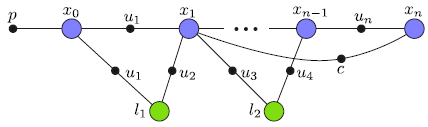
\includegraphics{SLAMFactorGraph.png}
		\caption{SLAM as a Factor Graph. The value $\mathbf{p}$ denotes a prior; $\mathbf{x_n}$ denotes the state vector; $\mathbf{u_n}$ denotes odometry measurements; $\mathbf{c}$ denotes close loops; $\mathbf{l_n}$ denotes landmark positions.}
		\label{fig:slam1}
	\end{figure}
	
	\paragraph{}
	The graph shown in Figure \ref{fig:slam1} is a Factor Graph representation of the dependencies between variables and measurements. A probabilistic framework can then be extracted from it. 
	\begin{equation}
	P(X,L,U,Z)\ \propto \ P(x_0)\prod_{i=1}^{M}P(x_i|x_{i-1}, u_i)\prod_{k=1}^{K}P(z_k|x_{i_k},l_{j_k})
	\label{probSLAMeq}
	\end{equation}
	\paragraph{}
	The general goal of probabilistic SLAM is to find variables $\mathbf{X^*}$ and $\mathbf{L^*}$ that maximizes the posterior probability distribution $P(X,L\ |\ U, Z)$ of the Equation \ref{probSLAMeq}. Two models of the probabilities given above are used commonly in SLAM to tackle this problem: the Process Model (also known as Motion Model in mobile robotics) and Observation Model:
	
	\begin{minipage}{.48\linewidth}
		\centering
		\begin{equation*}
		\begin{split}
		\mathbf{Process\ Model:} \\ 
		x_i = f(x_{i-1}, u_i) + w_i
		\end{split}
		\end{equation*}
	\end{minipage}
	\begin{minipage}{.48\linewidth}
		\centering
		\begin{equation*}
		\begin{split}
		\mathbf{Observation\ Model:} \\ 
		z_i = h(x_{i_k}, l_{j_k}) + v_k
		\end{split}
		\end{equation*}
	\end{minipage}
	
	\paragraph{}
	where $w_i$ is white noise with covariance $Q$ and $v_k$ is white noise with covariance $R$. The process (motion) model is usually a generalization of how the robot moves (kinematics) \cite{Montemerlo02fastslam:a}\cite{772544}. The observation model is a probabilistic representation of the performance of the sensors used to collect the data. Notice that both models are probabilistic and thus define the probability distributions $p(x_i|x_{i-1},u_i)$ and $p(z_k|x_{i_k},l_{j_k})$.

	\paragraph{}
	Under this framework, the mathematical analysis of SLAM has been shown that it is indeed feasible to build a nondivergent map with no prior information, so it is widely accepted that in theoretical grounds, SLAM is a solved problem \cite{SLAMPartI}\cite{Cadena}\cite{CsorbaThesis}\cite{938381}. However, there are computational and algorithmic challenges that hinders the development of a real-time implementation system that performs SLAM. This problem gets even more complicated when considering unstructured environments and large scale maps \cite{SLAMPartII}.
	
	\paragraph{}
	There are three main implementations of SLAM: Kalman Filtering and Extended Kalman Filtering (with early works such as proposed by R. Smith \cite{Smith:1990:EUS:93002.93291}), Particle Filtering (most notably with FastSLAM \cite{Montemerlo02fastslam:a}) and Information Filter (with the now state-of-the-art work of iSAM from Michael Kaess \cite{Kaess08tro}).

	\subsubsection{Kalman Filtering}
	\paragraph{}
	As one of the first implementations to appear to solve the problem of SLAM, the Extended Kalman Filtering (EKF) approach makes two approximations when formulating the probabilistic SLAM: both the Process Model and the Observation Model are linearised about a suitable linearisation point $\hat{x}$.

	\paragraph{}
	 Subsequently, the probability distributions $p(x_i|x_{i-1}, u_i)$ and $p(z_i|x_i, l_i)$ are modelled as Gaussians with the mean as $\nabla f|_{x=\hat{x}}$ and $\nabla h|_{x=\hat{x}}$ and covariances $Q$ and $R$. With this framework in place, a recursive two-step method can be found to update the posterior probability distribution at every iteration \cite{SLAMPartI}:
		\begin{equation*}
		\mathbf{Prediction\ Phase:}\ \ 
		P(x_{i},L|Z_{0:i-1}, U_{0:i}) = \int P(x_i | x_{i-1}, u_{i}) P(x_{i-1}, L |Z_{0:i-1}, U_{0:i-1})dx_{i-1}
		\end{equation*}
		\begin{equation*}
		\mathbf{Update\ Phase:} \ \  P(x_i, L | Z, U) = \frac{P(x_{i}, L | Z_{i-1}, U)P(z_i|x_i,L)}{P(z_i|Z, U)}
		\end{equation*}	 	
	\paragraph{}
	The Prediction Phase concerns the motion model, where an update of the estimated position of the mobile robot is made taking into account only the controls and kinematics of the robot itself. This is followed by an Update Phase, where the position of the robot is recalculated based oan the observation of a landmark, for example. This algorithm is then recursively applied for every time-step $i$. 	
	\paragraph{}	 
	 Since the product of two gaussians is a gaussian, the probability density function $p(x_i, L|Z, U)$ will remain Gaussian at all times, and a closed loop solution using just the mean and the covariance matrices can be found \cite{772544}.
	\paragraph{}	
	 Analysis of the EKF algorithms have shown that due to linearisation of the functions $f$ and $h$, assumptions about Gaussian Process and Observation Model can cause the EKF solution to perform poorly unless many loop closures are detected in frequent intervals \cite{doi:10.1177/1729881416669482}.


	\paragraph{}
	It is also known that the Kalman Filter approach requires storage of the order of $O(N^2)$ (where $N$ is the number of features), and for a classic implementation of the algorithm, it also requires computational power of the order of $O(N^2)$ \cite{CsorbaThesis}. New methods for computing the covariances (which cause the squared dependence) by exploring state augmentation, partitioned updates and sparsity in the matrices have demonstrated faster solutions, thus requiring less computational power \cite{SLAMPartII}.

	\subsubsection{Particle Filtering}
	\paragraph{} 
	In order to avoid linearisation of non-linear models, Particle Filtering (PF) has been a popular method to integrate non-gaussian distributions in the estimation \cite{Montemerlo02fastslam:a}\cite{772544}. The basis of particle filtering comes from Dallert's proposal of a Monte Carlo Localization (MCL) algorithm \cite{772544}. In sampling methods, the probability distributions are defined in function of the density of particles along the distribution. This approach avoids the assumption of linearity and Gaussian distribution, which makes this algorithm embrace multi-modal distributions.
	
	\paragraph{}
	Just like the EKF solution, there are many ramifications of PF methods. However, most of them follow the basic structure of the FastSLAM algorithm \cite{Montemerlo02fastslam:a}. This algorithm breaks the SLAM problem in one of localization over the robot's path, and $k$ of landmark location, where $k$ is the number of landmarks. The Localization problem is solved using MCL, which is composed of two parts \cite{772544}:
	 
	 \paragraph{Prediction Phase:} In this part, $N$ number of particles are drawn from the Motion Model distribution, whose density asymptotically represents the proposal distribution $P(X, L | Z_{0:i-1}, U)$.
	 
	 \paragraph{Update Phase:} Each particle from the Prediction Phase is then given a weight which is equal to the likelihood of the particle being there given the observation. In other words, $weight = P(Z|X, L)$, which is drawn from the Observation Model.
	 
	 \paragraph{}
	 After those two phases, the Landmark Location is solved using the classical EKF algorithm.
	 
	 \paragraph{}
	 Particle filtering methods have advantage over the EKF for not making any assumptions about linearity or Gaussianity of the distribution. Also if implemented wisely, it can reach $O(Mlog(K))$ time, where $M$ is the number of particles and $K$ is the number of landmarks \cite{Montemerlo02fastslam:a}.
	 
	 
	
	\subsubsection{Information Filter}
	\paragraph{}
	Information Matrices formulations of the SLAM algorithm is a technique used to compensate the quadratic dependency in computation time of the EKF by exploiting the sparsity in the Information Matrix.
	\paragraph{}
	It is known that the Dense Covariance Matrix in the EKF is the key to a convergent solution \cite{SLAMPartI}. However, this dense matrix means that the EKF will need computational power increasing quadratically in the number of landmarks.
	
	\paragraph{}
	By adopting an information matrix formulation of the EKF (the Information Matrix is defined as the inverse of the covariance matrix, or equivalently the coefficient matrix of the least square problem), this can be reduced to constant time computation \cite{doi:10.1117/12.381658}. This formulation is exactly equivalent to the EKF, with the advantage of being computationally advantageous \cite{Dellaert-2006-9639}.
	
	\paragraph{}
	The Information Filtering and Information Smoothing approaches have had many ramifications (with special mention to the Sparse Extended Information Filter (SEIF)\cite{doi:10.1117/12.381658}. The main algorithm that was developed was the iSAM (Incremental Smoothing and Mapping) \cite{Kaess08tro}, which is the one used in this project for being light and computationally advantageous.	
	
	\subsection{Stereo Visual Odometry}
	\paragraph{}
	Visual Odometry concerns the problem of estimating the robot's pose using its camera sensors. When two calibrated cameras are used, it is called Stereo Visual Odometry. It is a useful estimation procedure that can substitute wheel (kinematics) odometry in cases it is not available or it is not accurate (e.g. in rough terrain where the wheels slip).
	
	\paragraph{}
	The standard Stereo Visual Odometry algorithm works as follows \cite{StereoVis1}:
	\begin{enumerate}[leftmargin=.8in]
	\item Preprocessing Images: rectify images so that epipolar lines are aligned in left/right images; smooth images with an edge preserving filter such as the bilateral filter; calculate disparity map, by Block Sum of Absolute Difference (SAD) or equivalent, which indicates the inverse range map.
	\item Detect Features: use either Harris \cite{Harris}, FAST \cite{FAST} or  SIFT \cite{SIFT} for example, to extract features in the images.
	\item Match Features: by using a Score Matrix from the disparity map.
	\item Estimate Motion: by means of re-projection and triangulation of the calibrated cameras.
	\end{enumerate}
	
	\paragraph{}
	Stereo Visual Odometry is relatively accurate when cameras are properly calibrated, and results of the order of 0.25\% accuracy over 400m have been achieved using only the pure algorithm \cite{StereoVis1}. The tool used in this project was fovis \cite{fovis}, which is described in \cite{VisualOdometry}.
	
	\subsection{Iterative Closest Points (ICP)}
	\paragraph{}
	The problem that ICP is trying to solve: given a point cloud in a sensor coordinate frame that is a subset of a complex shape of another point cloud in a model coordinate frame, what is the translation and the rotation that aligns, or registers, the clouds by finding the minimum of a distance metric?
	
	\paragraph{}
	Given a point cloud in the sensor reference frame $P = \{p_1, p_2, p_3 ... p_{N_p}\}$, which is a subset of the point cloud in the model reference frame $X = \{x_1, x_2, x_3, ... x_{N_x}\}$, and assuming that the correspondence $P$ to $X$ is known and is $C = \{(x_1,p_1), (x_2,p_2), ... , (x_N, p_N)\}$, the minimum square error be formulated with the following equation:
	
	\begin{equation}
	f(\mathbf{\overrightarrow{q}}) = f(\mathbf{R},\overrightarrow{q_t}) = \frac{1}{N}\sum_{i=1}^{N}{||\overrightarrow{x_i}-\mathbf{R}(\overrightarrow{q_R})\overrightarrow{p_i}-\overrightarrow{q_t}||^{2}} 	
	\label{eq:ICPObjective}
	\end{equation}		
	
	\paragraph{}
	Equation \ref{eq:ICPObjective} is a function of the Rotation Matrix $\mathbf{R}$ and the translation vector $\overrightarrow{q_t}$. It is computationally cheaper to define the Rotation Matrix as a function of the quaternion $q_R$, as it only requires 4 variables instead of the 6 needed for the Rotation Matrix. If we define the vector $\overrightarrow{q} = [\overrightarrow{q_R} | \overrightarrow{q_t}]^T$, then we can optimize the above as a function of the 7 variable vector $\overrightarrow{q}$ \cite{AMethodRegistration}. This vector would then define a translation from $P$ to $X$ that would minimize the objective function.
	
	\paragraph{}
	Using that equation, the ICP algorithm can be implemented using the following iterative operation:
	\begin{enumerate}[leftmargin=.8in]
		\item Find the correspondences between points $X$ and $P$ by evaluating closest points in each of the points of the smallest set.
		\item Compute the registration by finding $\underset{\overrightarrow{q*}}{min}f(\overrightarrow{q})$ and apply the transformation to the whole set $P$.
		\item If $f(\overrightarrow{q*}) \leq \tau$, where $\tau$ is a threshold value, then stop. Otherwise go back to step one.
	\end{enumerate}	
	
	\paragraph{}
	The ICP algorithm formulated with the above objective function always converges monotonically to the nearest local minimum \cite{AMethodRegistration}. The global minimum is more difficult to find, since it depends on the relative initial pose of the model and the sensor reference frames. Thus, given an adequate set of initial translation and rotation, one can globally minimize the mean-square distance over all six degrees of freedom \cite{AMethodRegistration}.

	\paragraph{}
	Since first formulated, a number of variants of the ICP appeared. They are usually alternative ways of selecting subsets of the points, finding correspondences, weighting correspondences, rejecting specific pairs, assigning an error metric, computing the minimum of the objective function, or a combination of those \cite{ICPVariants}. The variant used in the project was the AICP, which rejects point correspondences based on the overlap between point clouds \cite{7989547}.
	
	\subsection{3D Reconstruction Systems}
	\paragraph{}
	Although point clouds can be very useful for tasks such as correction of poses, they do not provide for higher level of scene understanding. 3D Reconstruction Systems are used for that: given discrete data from a sensor, the 3D Reconstruction System tries to recreate the scene geometrically by estimating surfaces and occupancy, and graphically by providing texture.
	
	\begin{wrapfigure}{h}{0.6\textwidth}
		\centering
		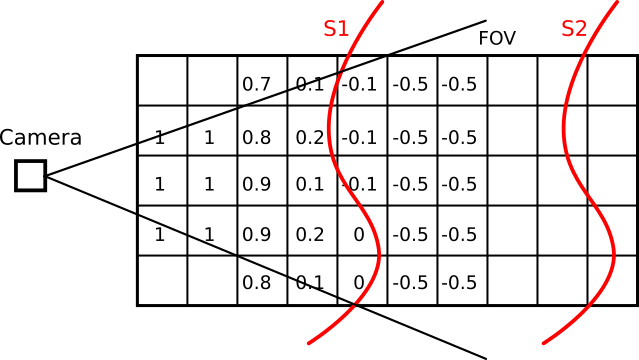
\includegraphics[width=0.55\textwidth]{TSDF}
		\caption[t]{Graphical representation of a voxel grid. Each Grid has a Truncated Signed Distance Function value corresponding to the distance to the nearest surface. In order to avoid interfering with other surfaces, the value assignment to voxels that are far away are taped off after a few voxels}
		\label{fig:TSDF}
	\end{wrapfigure}
	
	\paragraph{}
	In order to represent surfaces, there have been a couple of algorithms that have been used. The most popular one uses the idea of Signed Distance Functions (SDF), which is a scalar function that represents distances to the nearest surface.Given known poses and depth images, the world is modelled as a voxel grid in which each voxel holds  a value that represents its distance from the closest surface. Positive numbers mean that the voxel is outside the surface and negative values means that the voxel is inside the function. The voxel grid then represents isosurfaces which can be extracted in polygon meshes using an algorithm such as the Marching Cubes \cite{marchingcubes}.
	
	
	\paragraph{} This method of representing the world is very flexible, even though memory intensive. Modern approaches have adopted the concept of the Truncated Signed Distance Function (TSDF \cite{TSDF}), in which the voxel values are truncated to avoid interference with other surfaces (see Figure \ref{fig:TSDF}).
	
	\paragraph{}
	There are mainly three classes of reconstruction systems that can be divided:
	\begin{itemize}
		\item Active vs Passive Sensors: when using an active sensor (such as Kinect to get RGB-D images), the depth estimates are accurate enough so that a simple fusion using weights is enough to get a good reconstruction (example system KinectFusion \cite{kinectfusion}); when using a passive sensor (such as in DTAM \cite{DTAM}), the depth estimates are usually less accurate and thus there is a need to use a regularizer
		\item Object-Centric vs Mobile-Robot-Centric Fusion: when in an object-centric situations, it can be assumed that the voxel block and the voxel grid will be seen all of the time by the sensors (such as in KinectFusion \cite{kinectfusion}). Also, the object is seen in loops multiple times, thus allowing for fine detailed reconstructions; this is not true for a mobile-robot-centric situation, where the robot navigates through the scene instead of around it, and new voxel blocks have to be dynamically allocated depending on the robot's trajectory (such as in Kintinuous \cite{kintinuous}, even though it still uses fixed voxel blocks). It is also unlikely that the same scene is going to be seen multiple times in a range of different angles.
		\item Large vs Small Scale: memory allocation plays a huge part when large scale models are used, and that comes at a cost of usually higher voxel sizes, whereas in small scale very small voxel sizes and details can be preserved. Systems that took memory in consideration is the Hashing Voxel Grid (HVG) \cite{HVG}
	\end{itemize}
	
	\paragraph{}
	Due to the RGB-D sensor becoming widely available as a commodity, most 3D reconstruction systems have focused on hand-held devices for small scale reconstruction. Since this project relies on LiDAR data, a new system has been chosen.	
	
	\paragraph{}
	The system used in this report is BORG-CUBES, which is a reconstruction system that uses sensor-agnostic voxel grids to reconstruct the system. Since LiDAR data come at way less frequency than RGB-D data, BORG-CUBES relies on a prior regularizer to improve the quality of the reconstruction. It can also integrate stereo visual images, which gives data in higher rates but provide a much lower quality depth map than using LiDAR.
	
	\subsection{Past Work on 3D Reconstruction using LiDAR}
	

	\newpage
	\section{System Pipeline} \label{pipeline}
	\paragraph{}
	The pipeline for the overall system can be seen below. It consists of 4 modules: (I) First odometry estimates (based on either Visual Odometry or Wheel Odometry); (II) Laser Odometry (using AICP \cite{7989547}); (III) Loop closure detection and Graph Optimization (using iSAM \cite{Kaess08tro}); (IV) 3D dense volumetric reconstruction (using BOR\textsuperscript{2}G-CUBES \cite{TannerFSR2015}\cite{TannerArXiv2016}).

	\paragraph{}
	These 4 modules are broken down in two parts: the first part is concerned about solving the SLAM problem, which outputs a reliable trajectory and map. The second part is concerned about inputting that to a 3D reconstruction system (which in this case if BOR\textsuperscript{2}G-CUBES) to build the environment volumetrically. Figure \ref{fig:SystemPipelineFigure1} shows the overall system built.
	\begin{figure}[h]
		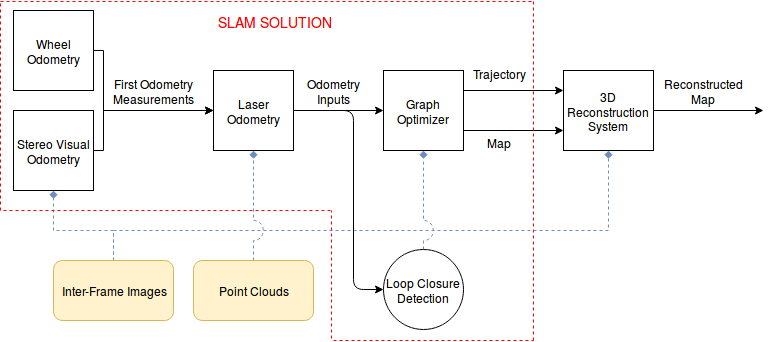
\includegraphics[width=\linewidth]{SystemPipeline}
		\caption{Diagram of the overall system pipeline. The beige boxes represent data collected from a sensor, the white boxes represent data being processed and the output being input to the next box. The rounded box is a module built for data association.}
		\label{fig:SystemPipelineFigure1}
	\end{figure}
	
	\paragraph{}
	The data was collected using a LiDAR sensor (MultiSense SL or Velodyne) to get the Point Clouds at every iteration.
	\newpage
	\section{SLAM Solution}
	\paragraph{}
	As already introduced in Section \ref{pipeline}, the SLAM solution has 4 independent building blocks. This offers flexibility enough to test the effect that each part has in the outcome of the map. This section is going to discuss deeper how the solution works with all the building blocks working together. 
	 
	\subsection{First Odometry Measurements}
	\paragraph{}
	The first odometry measurements offer a relatively inaccurate estimation of the pose of the robot at a certain time. The purpose of these first estimates is to give an input pose to the Laser Odometry algorithm to perform a better estimate of the trajectory. As shown in Equation \ref{eq:ICPObjective}, the ICP algorithm requires the initial pose of the reference frame of the two point clouds, denoted $X$ and $P$ in Section 2.

	\paragraph{}	
	Depending on how accurate those poses are, the ICP algorithm can find a global minimum (or get close to it) and offer a fine-tuned estimate of the trajectory. It is important then to get the first odometry measurements as accurate as possible, so that the Laser Odometry can always find a global minimum and make the trajectory optimum.
	
	\paragraph{}
	During the project, two methods to get the first odometry measurements were used. When getting data with the mobile robot Husky \cite{Husky}, the wheel odometry provided by the system served as a good first estimate of its position. When getting the data with the MultiSense SL \cite{multisense}, Stereo Visual Odometry from MultiSense's stereo camera was performed to get the first odometry estimations.
	
	\subsubsection*{Stereo Visual Odometry}
	\paragraph{}
	The Stereo Visual Odometry used is based on the system described at \cite{VisualOdometry} and implemented with the fovis library \cite{fovis}. Figure \ref{fig:VisualOdometry1} shows one frame of the result of the visual odometry system when applied to the dataset collected for this project. The inputs came from the stereo camera in the MultiSense SL, collected at 30Hz in a relatively illuminated indoors scenario.
	
	\paragraph{}
	There are a couple of important details that have to be taken into account when implementing the Stereo Visual Odometry. First, the estimates are usually worse than using wheel odometry. This is the case because there are much more variables involved in this system: blur of the image (which can affect selection of key frames), capture time of images, processing time to get and match point features, and velocity of the sensor. 
	
	\paragraph{}
	Secondly, the VO usually drifts on the z direction, and on the pitch and roll directions. Since the trajectories for this project were mainly across one floor, with flat terrain and mainly two dimensional, the z displacement and the pitch and roll variations were set to zero. The result is a much more accurate 3D map than the one that would be obtained if the 6DOF were being estimated.
	
	\paragraph{}
	It is very common to use a combination of Visual and Inertial sensing to get a more accurate estimation of pose. The purpose of using both is that they offer complementary characteristics, mainly with the Inertial system correcting the Euler Angles and vertical displacement of the visual estimation. Many examples of such systems can be observed, such as in [LACKING REFERENCES].
	
	\begin{SCfigure}[][ht!]
	\begin{minipage}{0.65\textwidth}
		\centering
		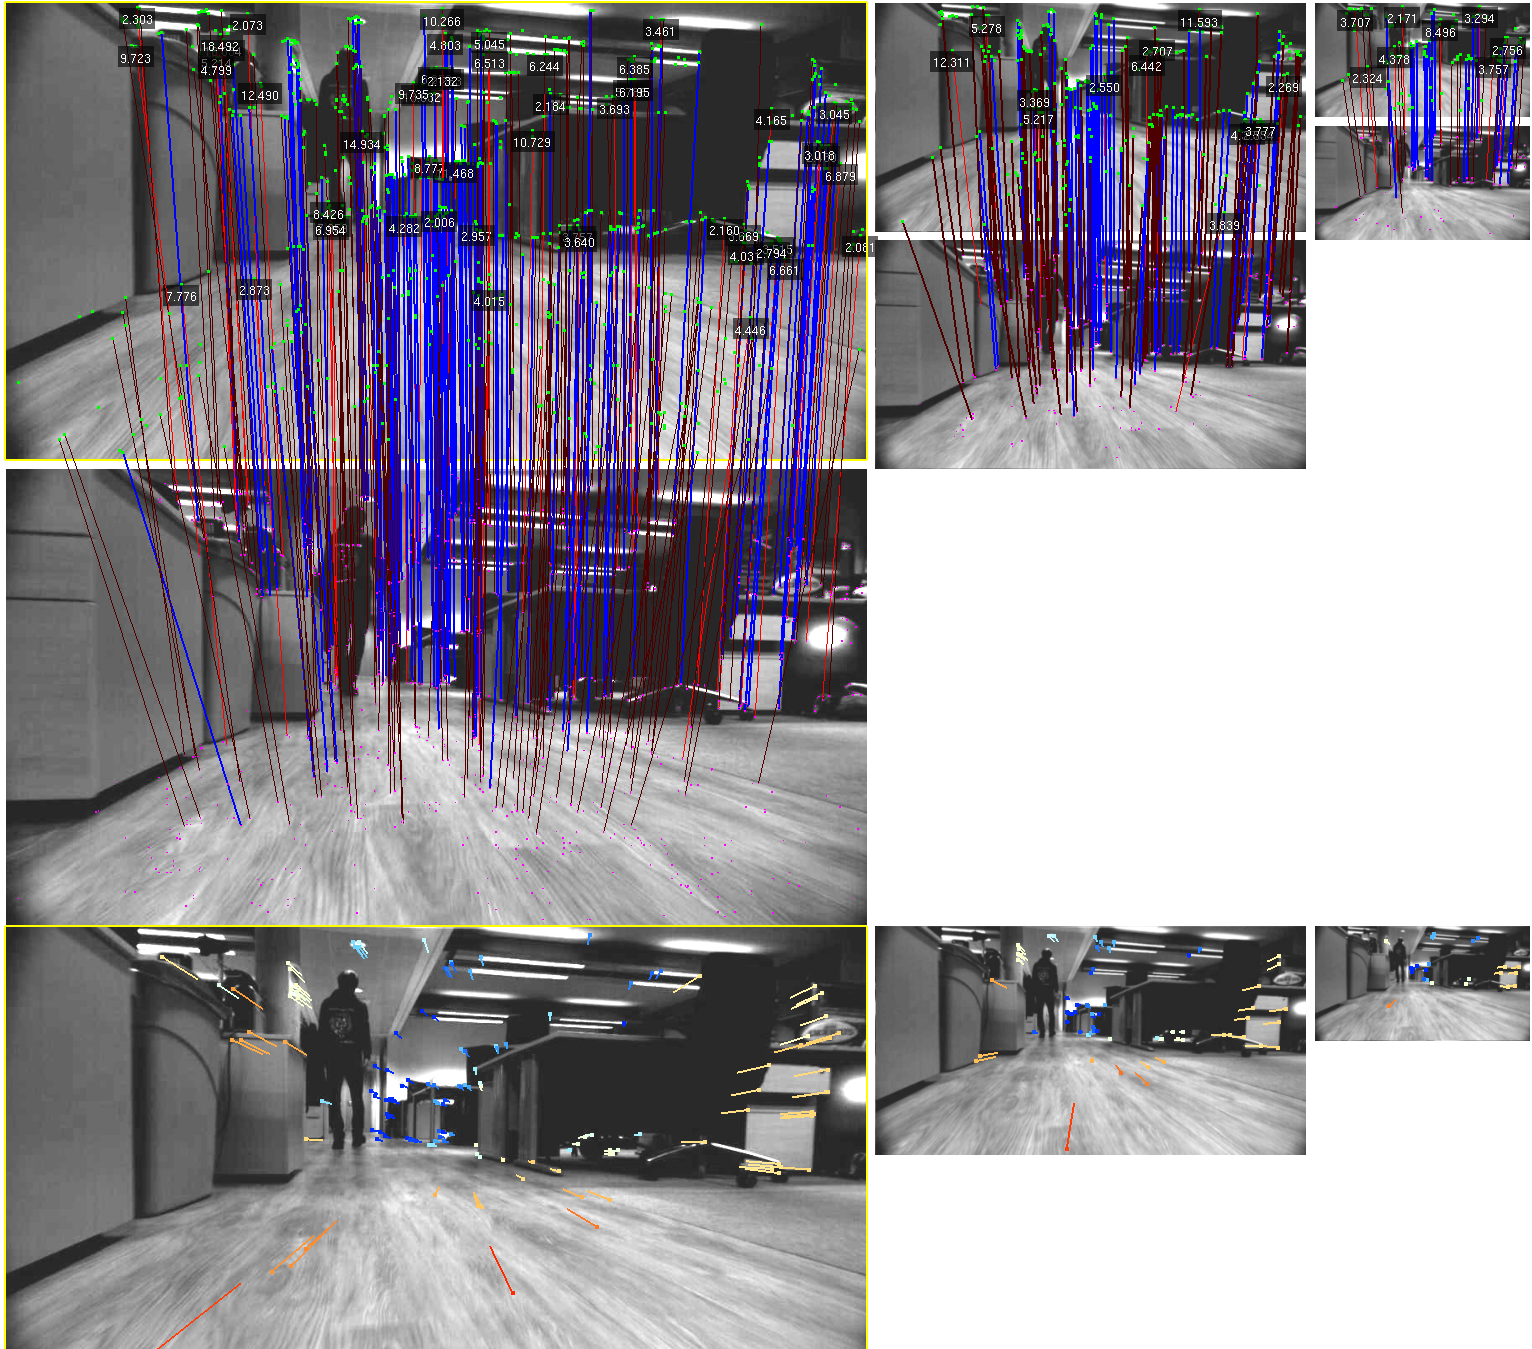
\includegraphics[width=\textwidth]{VisualOdometry1}
	\end{minipage} \hfill
	\begin{minipage}{0.35\textwidth}
		\centering
		\caption[t]{Result of fovis library to the data collected at the Information Engineering Building at University of Oxford. The first row of images show a Gaussian Pyramid to extract point features. The Key Frame is shown in the second row where features extracted are matched back to the first row images. Red lines indicate outliers and blue lines indicate inliers (bad and good correspondence respectively). The last row shows the result of the rotation matrix in the pictures. The scale of the movement is indicated as a colour scale from blue to red.}
			\label{fig:VisualOdometry1}	
	\end{minipage}				
	\end{SCfigure}
		
	\paragraph{}
	An Inertial Measurement Unit (IMU) was not available at the time of the experiments taken for this project, so such a combination could not be implemented. However, restricting the estimations to two dimensions led to similar results. Further advancements in the project would include having an IMU to make the estimation free in the 6DOF instead of restricting it to 3DOF.
	
	\subsubsection*{Wheel Odometry}
	\paragraph{}
	Remember to put the pictures of the Wheel Odometry and the corrected pose using AICP.
	
	\paragraph{}
	Just like with the stereo odometry and as common with systems based on proprioceptive sensors without loop closing mechanism, this method of locomotion drifts significantly. After applying this algorithm to the pose of the robot, the results of the 
	\paragraph{}
	Also a good idea would be to put the Wheel Odometry and the Visual Odometry as comparison using the same Dataset (the one that Simona Collected at Edinburgh would be perfect)
		
	\subsection{Laser Odometry}
	\paragraph{}
	Given the first odometry measurements, it is clear that the resulting map does not look right. In order to improve the estimate of the trajectory, the next step is to use laser based localization using the Point Clouds from the trajectories.
	
	\paragraph{}
	Since it uses an exteroceptive sensor, it is expected that laser based localisation achieves significantly less drift than using a proprioceptive sensor (like wheel odometry). However, since ICP algorithms are prone to failure depending on how inaccurate the first pose estimations are, there is a need to incorporate a robust method of incorporating laser based-localization.
	
	\paragraph{}
	For this reason, this project used the system described at \cite{AICPAlign} for laser odometry. This algorithm works in two phases: First it selects a point cloud to be the reference of registration. Second, it calculates the prediction of failure of subsequent point clouds to register with the reference. If the prediction states that there is no failure, then the point cloud is registered to the reference, and it iterates to the next point cloud. If the prediction states that there is a risk of failure, then the point cloud becomes the new reference of registration, and subsequent point clouds are registered to this new reference frame.
	
	\paragraph{}
	The risk of failure is calculated using two parameters: the alignability and the overlap. First the overlap is calculated using the volumetric overlap of the range and occupancy grid from the first odometry measurements. After that, the alignability is calculated, which is a measure of how "constrained" in three dimensions the two point clouds are. This is to avoid the problem of registering two point clouds taken in a long corridor for example, where there will be many local minima since the path would be unconstrained in one dimension. From those two parameters, a model is learnt using Support Vector Classifier (SVC), and the Risk Prediction is drawn from that model. More details can be checked at \cite{AICPAlign}.
	
	\paragraph{}
	Notice that the algorithm is robust to Euler Angles and Translation, and makes the short term drift significantly smaller. The main source of drift in this case is when it predicts high risk failure and have to change the reference of registration. This leaves a small amount of drift at every changing of reference, which accumulates in the long run and means a noticeable final drift.
	
	\paragraph{}
	The results for each of the paths are shown below for comparison. Figure \ref{fig:LaserOdometry1} shows the results for the data collected with Husky using Wheel Odometry. It is noticeable the difference between the accuracy of the First Odometry Measurements to the Laser Odometry. However, it can be seen that there is drift due to how the AICP algorithm works.
	\begin{SCfigure}[][ht!]
	\begin{minipage}{0.65\textwidth}
		\centering
		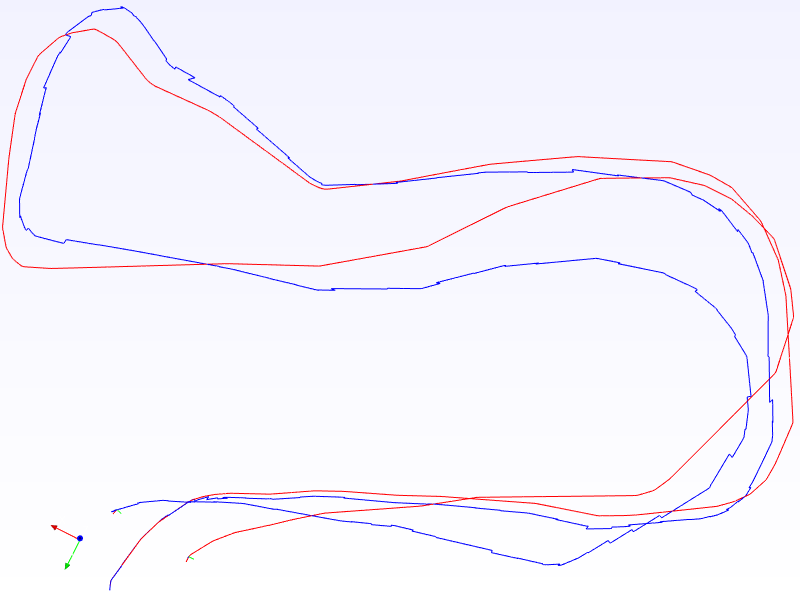
\includegraphics[width=\textwidth]{LaserOdometry1}
	\end{minipage} \hfill
	\begin{minipage}{0.35\textwidth}
		\centering
		\caption[t]{Result of the Wheel Odometry feeding the laser odometry system. The red path shows the Wheel Odometry and the green path shows the corrected poses after being computed by the AICP algorithm. Notice that the corrections are more obvious during the turns, when the wheel odometry is particularly inaccurate.}
		\label{fig:LaserOdometry1}	
	\end{minipage}				
	\end{SCfigure}
	\paragraph{}
	This accumulated drift is unnoticeable from frame to frame. However, over a long enough distance, the accumulated drift becomes significant. A way of correcting this long term distance is by using the idea of loop closures.
	
	\subsection{Loop Closure Detection}
	\paragraph{}
	In order to adjust for the accumulated drift of the path estimate, a loop closure detection algorithm was placed. Since it was assumed that the robot would not overdrift, three simple heuristics were used to detect loop closure: Time Filter Sampling, Euclidean Distance, and Pose Alignment. 
	\begin{itemize}
		\item \textbf{Filter Sampling:} In order to avoid the problem of loop closing two state estimates that are in the same room but did not leave the room, a time filter sampling was applied. The idea is to sample every $S$ state estimates, so that the candidate loop closing states would be sparse enough so that the loop just occurs between big time frames, but dense enough to apply euclidean distance.
		\item \textbf{Euclidean Distance:} Once the estimates have been  sampled, the euclidean distance between each of them is applied. If the distance between any two states is less than a threshold value $E$, then the two estimates form a candidate pair and they are added in the candidate pair list.
		\item \textbf{Pose Alignment:} After the resampling, the candidates pairs are tested for their relative pose. Since the loop closure correction relies on alignment of point clouds using ICP, it is a good strategy to select poses that would maximize the overlap between the point clouds associated with the candidates. In order to do that, another resampling is done based on the overlap between the field of view of the estimates. If the overlap is less than a threshold value $O$, then the candidate pair is dropped out from the list, and the remaining are the loop closures that are considered.
	\end{itemize}
	
	\paragraph{}
	The parameters $S$, $E$ and $O$ are chosen by hand depending on what dataset is used in the algorithm. Changing the parameters can affect the outcome of the map significantly, so it is important to spend some time tuning them to the specific requirements of the test.
	
	\paragraph{}
	Figure \ref{fig:loopClosureDetection} shows the results of the Loop Closure detection when applied to the Husky dataset. Due to the relatively low velocity of the mobile robot, the parameters were adjusted to match the time that the mobile robot would take to leave a room before coming back to the same room.
	\begin{SCfigure}
	\begin{minipage}{0.67\textwidth}
				\centering
				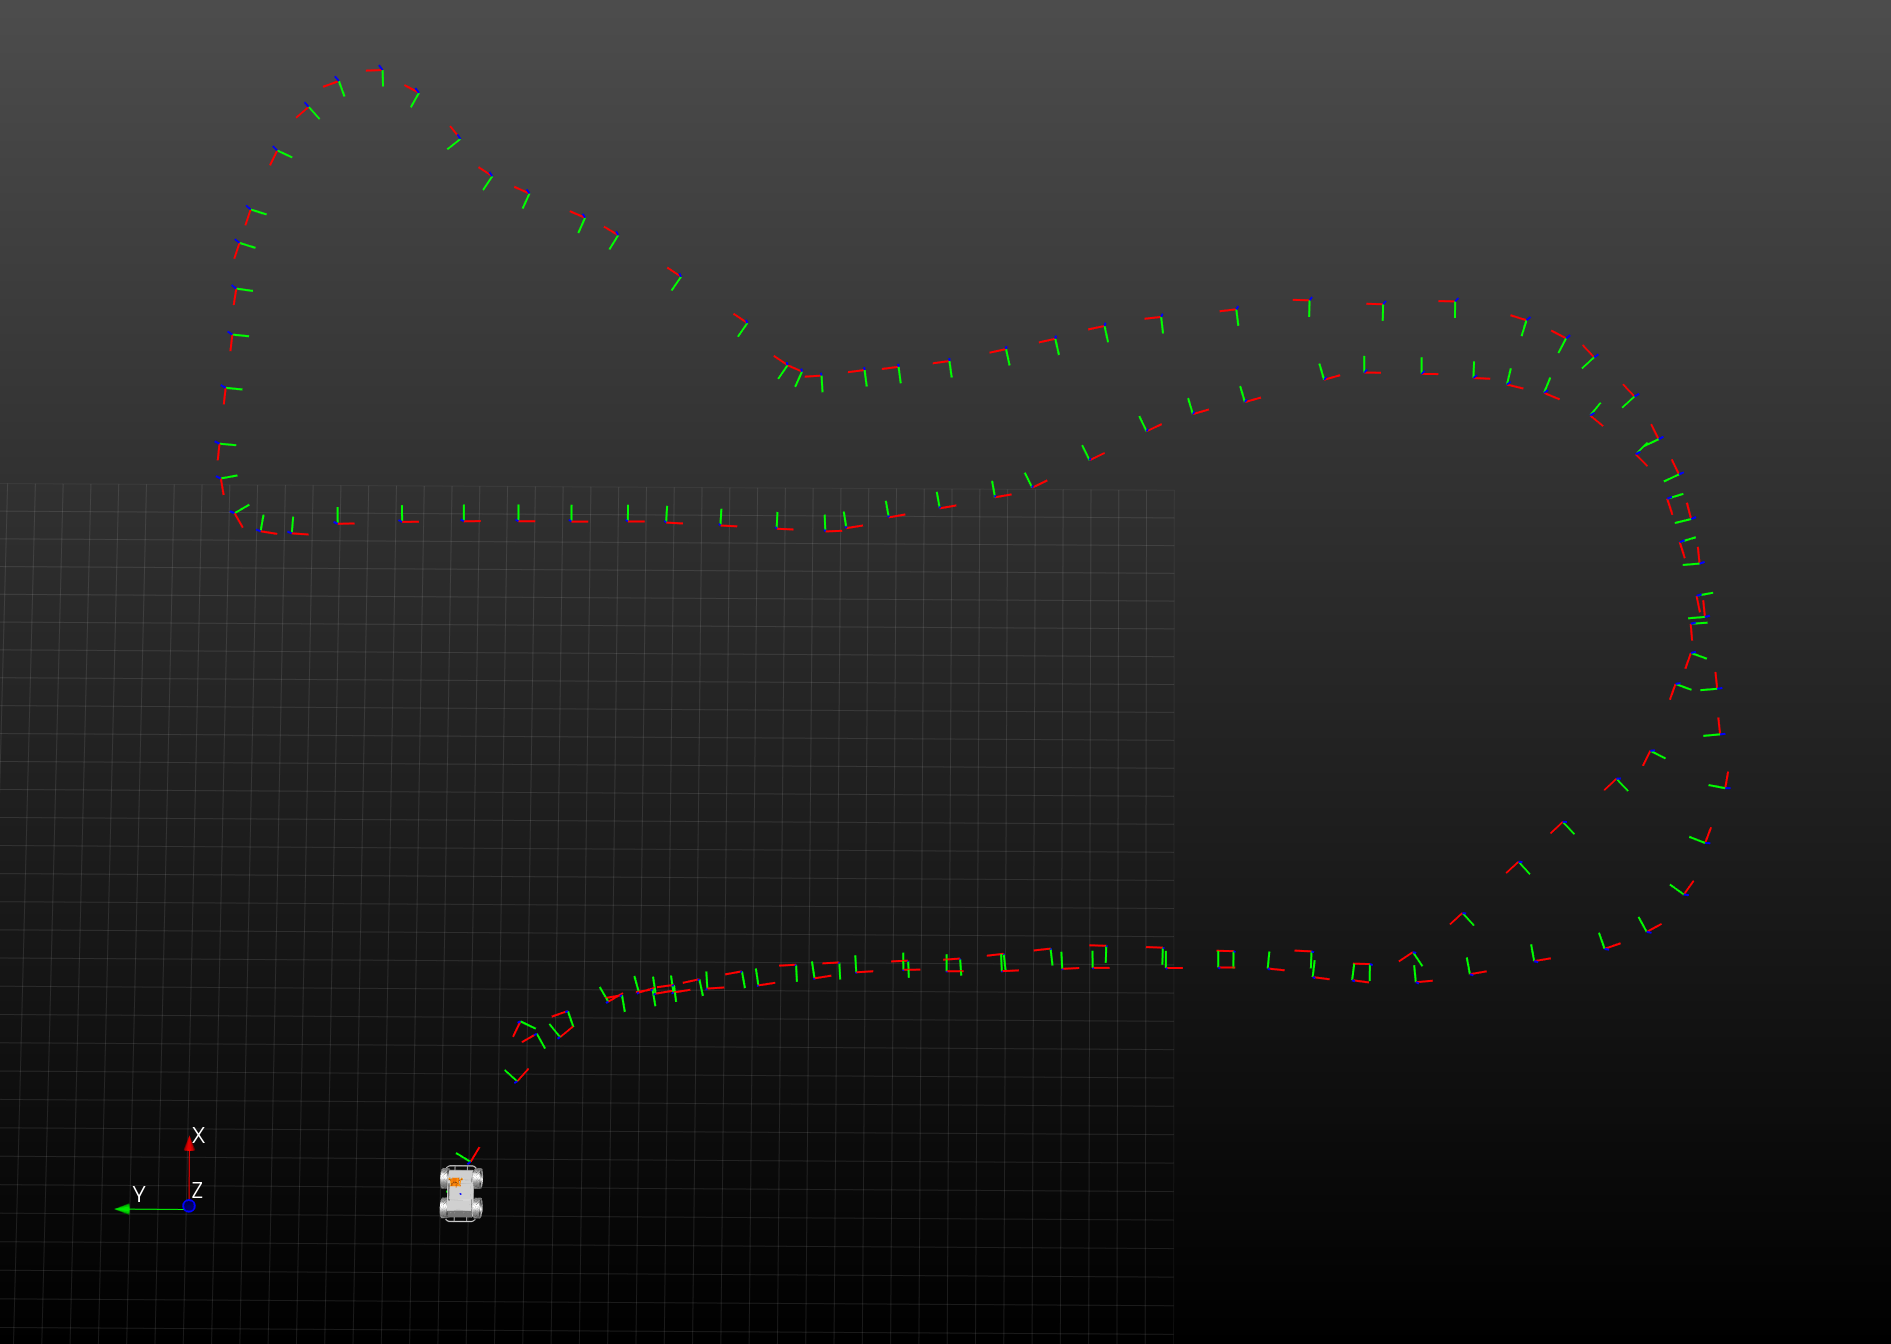
\includegraphics[width=\textwidth]{LoopClosureTimeSampling}
				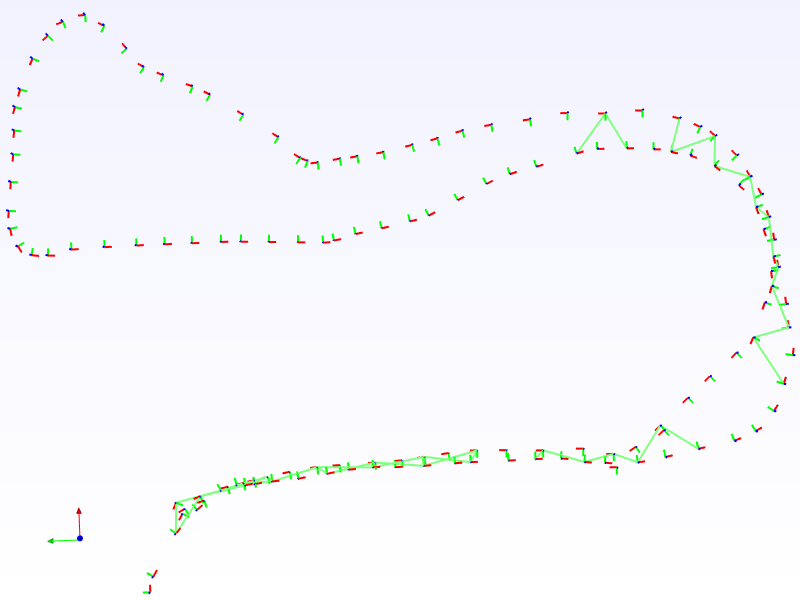
\includegraphics[width=\textwidth]{LoopClosureEuclideanSampling}
				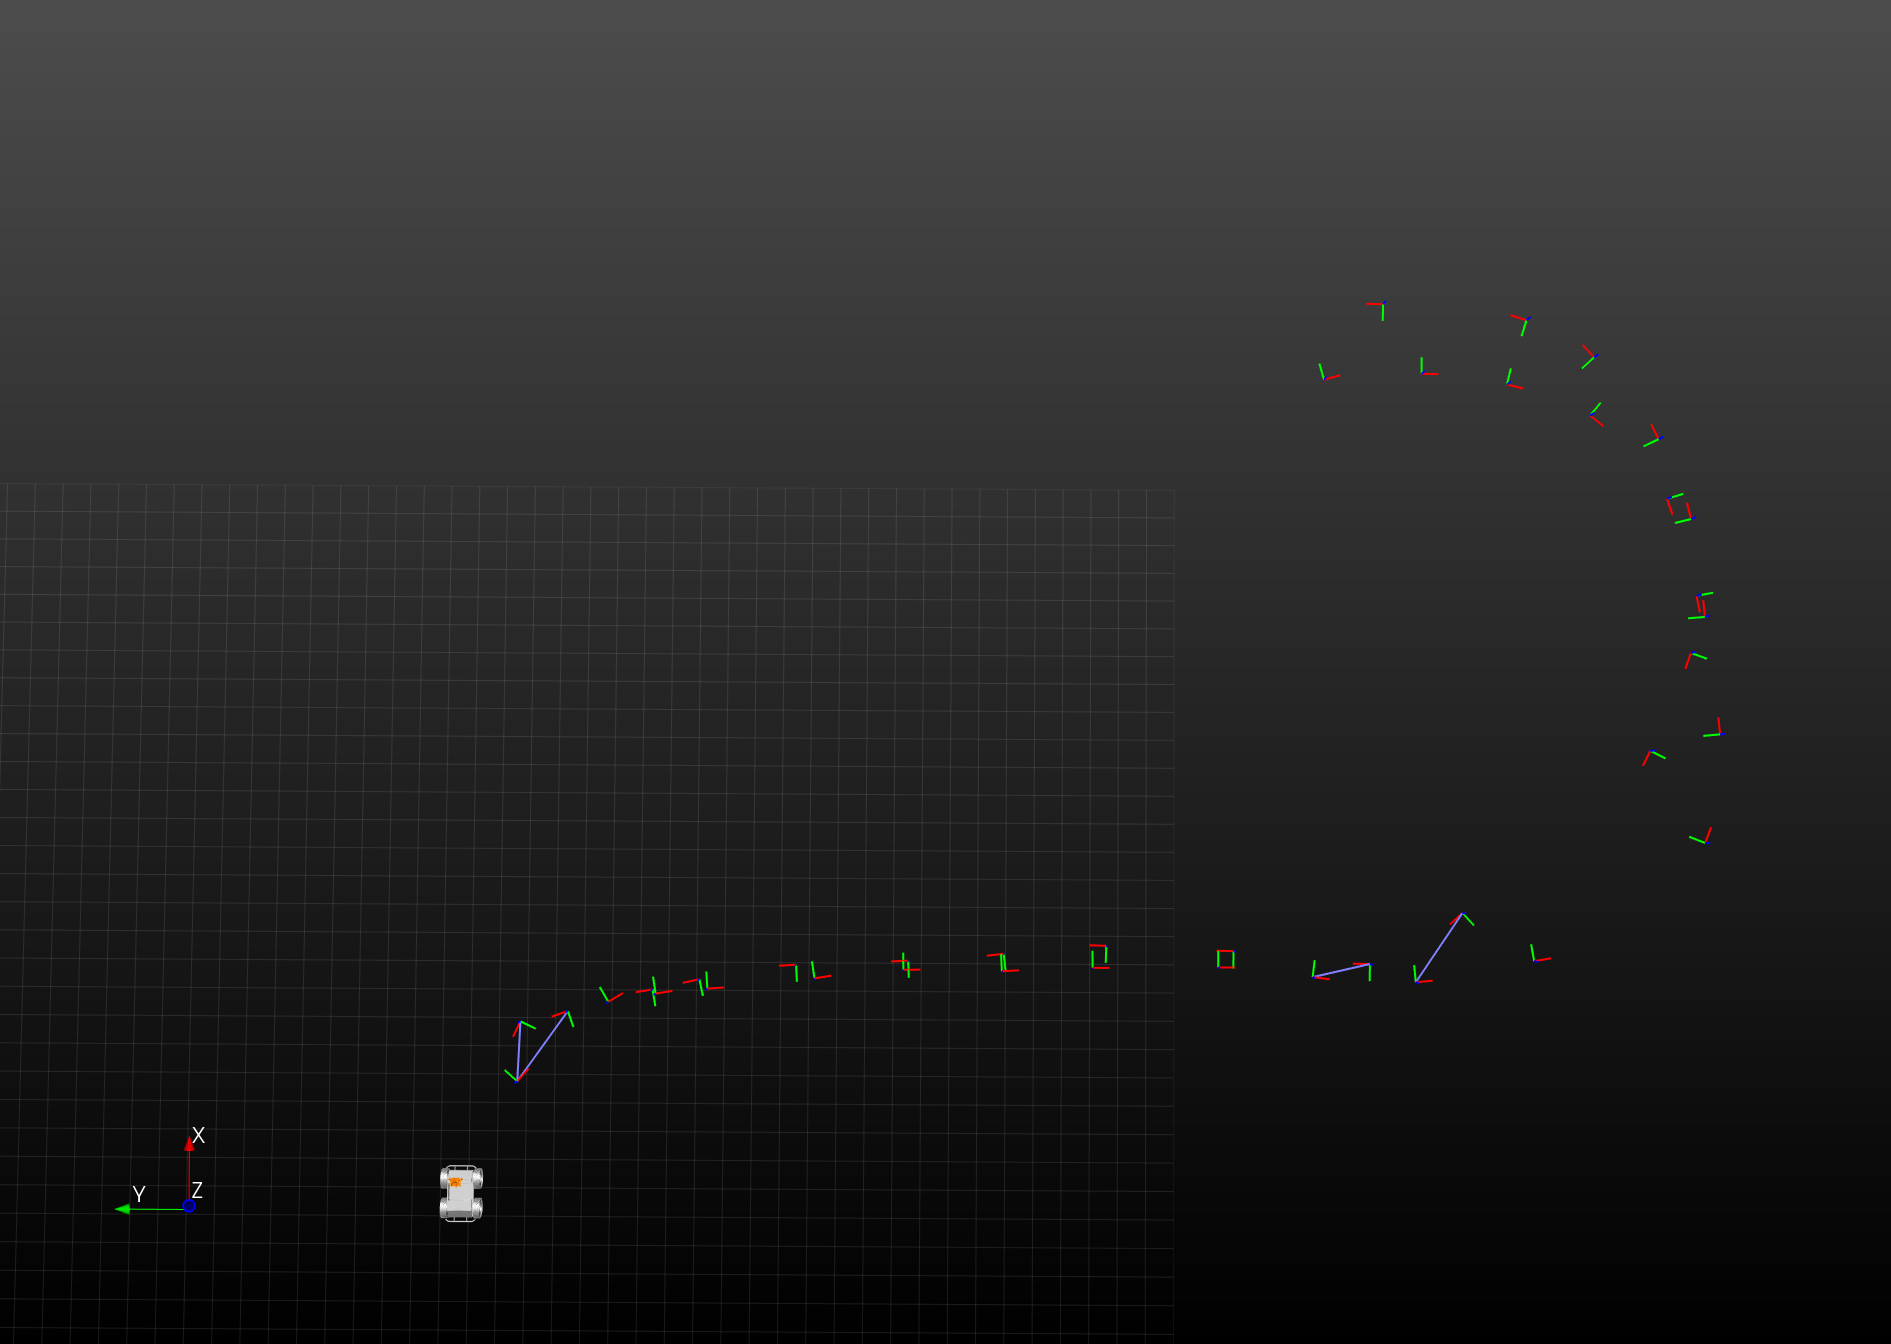
\includegraphics[width=\textwidth]{LoopClosureFinal}
	\end{minipage}\hfill
	\begin{minipage}{0.33\textwidth}
		\centering
		\caption[t]{The three heuristics for loop closure detection. Data shown was collected using the Husky Mobile Robot and the Velodyne LiDAR, visualized in bird's-eye view with red and green coordinates representing the path of the robot. The figure on the top shows the result of the time sampling. The plot in the middle shows the Euclidean Distance Pairings. The last figure is the result of the Pose (overlap) filter. In this experiment, $S=2$, $E=2$ and $O=0.5$.}
		\label{fig:loopClosureDetection}
	\end{minipage}
	\end{SCfigure}
	\paragraph{}
	It is also important to notice that marginally different parameters have an impact on the number of loop closures and on the outcome of the map. Figure X shows the results of different maps according to different settings of the loop closure parameters.
		
	\paragraph{FIGURE}
	
	\paragraph{}
	The assumption that the drift in two loop closures is relatively small is not always valid. For cases when the drift is sufficiently big, other methods for finding loop closures have to be implemented. A popular approach is to find loop closures from images, where each frame is compared given some descriptors and if two scenes look similar enough, they are considered as a loop closure. This is a more sophisticated and accurate system. However, since this project is concerned with indoors mapping, it is assumed that a substantial amount of loop closures will be available in a relatively short time frame. This validates the loop closure system used. Further work in this area would be necessary to make the system more robust to big drifts.	
	
	\paragraph{}
	Ideally, the number of loop closures should be neither too big nor too small. Loop closure can be thought of strings ``tightening" the Factor Graph in Figure \ref{fig:slam1} by adding constraints to it. If many loop closures are made, the graph becomes too constraint and new corrections to the map would be insignificant. This can be naively desirable since it means that the certainty of the graph is high, but if one loop closure is a bit off, then the effect cannot be corrected subsequently. In the other hand, if few loop closures are made, then the drift between poses are not corrected substantially and the overall error in the graph is high.
	
	\paragraph{}
	Therefore it is crucial to tune the parameters so that meaningful loop closures are selected. 

	\paragraph{Front End Loop Closing Problem.} One of the biggest problems with loop closing is that it has a massive effect on the topology of the map. If for some reason either the loop closure is not a good one or if the point cloud registration is innacurate, the effect on the map is disastrous.
	
	\paragraph{}
	Unfortunately, ICP algorithms are known for having multiple minima points, which means that not always the registration converges to the global minimum point. Even worse, sometimes the global minimum point might not even be the right registration, maybe due to ambiguities in the map (consider the long-corridor problem and registering a point cloud in the long-corridor).
	
	\paragraph{}
	This brought up the problem of multimodaility: since the ICP is not a convex function, there are multiple minima that might be the appropriate one. In the project, this was demonstrated by slightly perturbing the position of the robot in relation to the next. In the Figure X below, it can be seen that a small perturbation may make the ICP converge to another minimum point, which means that one of the is wrong. If the wrong registration point is the one detected by the algorithm, then it would introduce an almost irreversible error in the map, and make it more difficult to reconstruct it accurately in the 3D reconstruction system.
	
	\paragraph{}
	Many systems and algorithms could be used to avoid this problem, including multihypothesis and a stronger front end selection key. In the project, it was chosen to select the loop closure by hand due to the lack of time to implement a multihypothesis system. That is however an area that should be researched in future projects.
	\subsection{Graph Optimization}
	\paragraph{}
	As presented in section 2, many graph optimization tools were created (including g2o [NEED REFERENCE] and iSAM). In this projects, the Graph Optimization was conducted using the iSAM library. Since the exteroceptive model used was LiDAR data instead of any landmark localizer (like Visual Data or Fiducial Systems for example), a Pose-Only graph is generated. It is important to notice that all of the SLAM properties for landmarked based systems also hold for Pose-Only based systems [lacking citation].
	The results of the Wheel Odometry system when applied the Optimization are shown in the Figure \ref{fig:GraphOptimization1}.
	
	\begin{figure}[ht]
		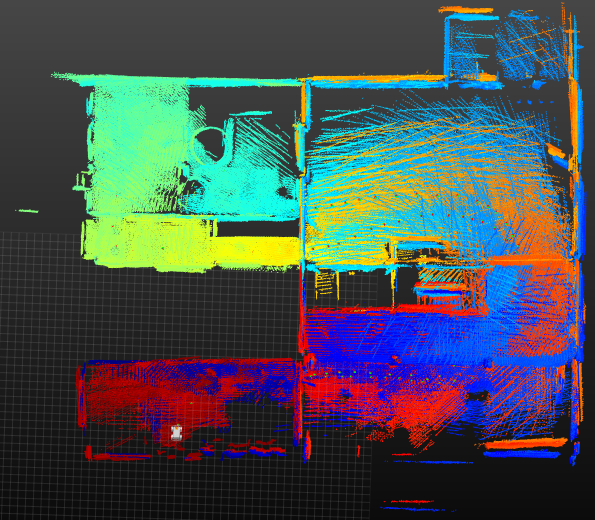
\includegraphics[width=0.45\textwidth]{ResultNoLoopClosure}
		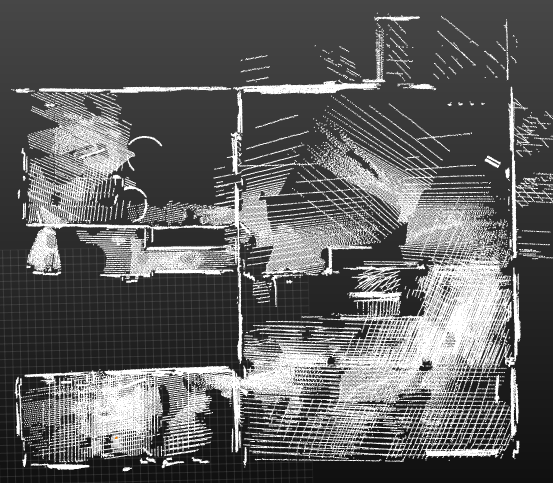
\includegraphics[width=0.45\textwidth]{ResultLoopClosure}
		\caption{Result of the Graph Optimization solution. The map in the left shows the Point Clouds collected without Graph Optimization and Loop Closures applied. The map in the right shows the result of the map after the loop closures have been implemented in the iSAM algorithm. Notice the alignment of the wall at the top of both images and at the very bottom to compare the overall drift of both systems. The point clouds in the picture in the left are coloured with timestamps.}
		\label{fig:GraphOptimization1}	
	\end{figure}
	\newpage
	\section{Integration with BOR\textsuperscript{2}G-CUBES}
	\paragraph{}
	As explained in section 3, the result of the Graph Optimization is then input to BORG-CUBES. Since this algorithm was built to reconstruct cities with an eye at autonomous driving, it expects a pretty dense representation of the LiDAR point clouds. Unfortunately, this is not the case for mobile robots operating indoors with a single 270 degrees sensor.
	
	\paragraph{}
	The BORG CUBES algorithm can be implemented in two modes: Regularized and Non Regularized. The regularization parameters is used to make the surfaces smoother, assuming that relatively inaccurate estimate of distances are drawn from the Visual Reconstruction or alternatively relatively inaccurate estimation of pose.
	
	\paragraph{}
	Even though regularizing the map yield a smoother reconstructed surface, it also excludes surfaces that are majorly disconnected from other surfaces, as can be seen in the next figures.
	
	\begin{figure}
		\centering
		\begin{tabular}{cccc}
		\subfloat{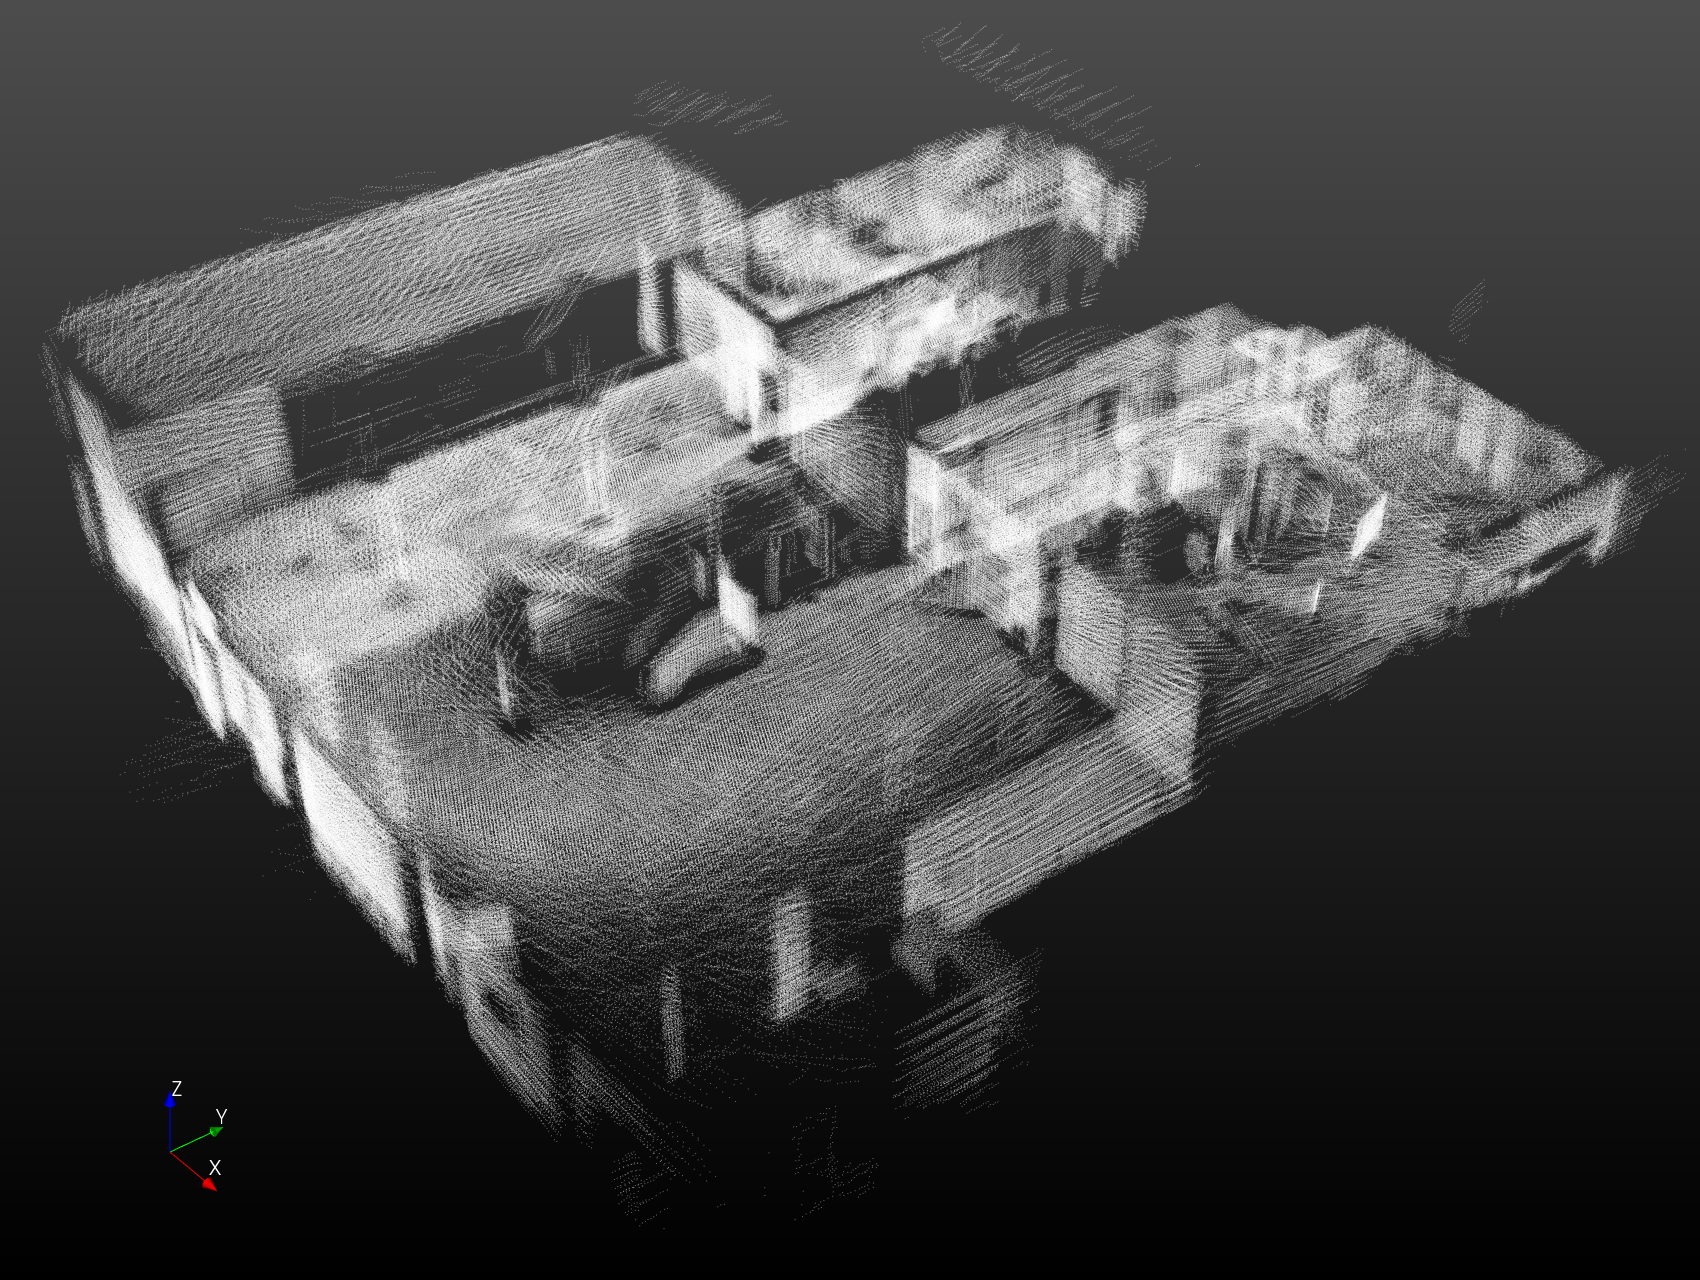
\includegraphics[width = 0.3\linewidth]{PTCL1}} &
		\subfloat{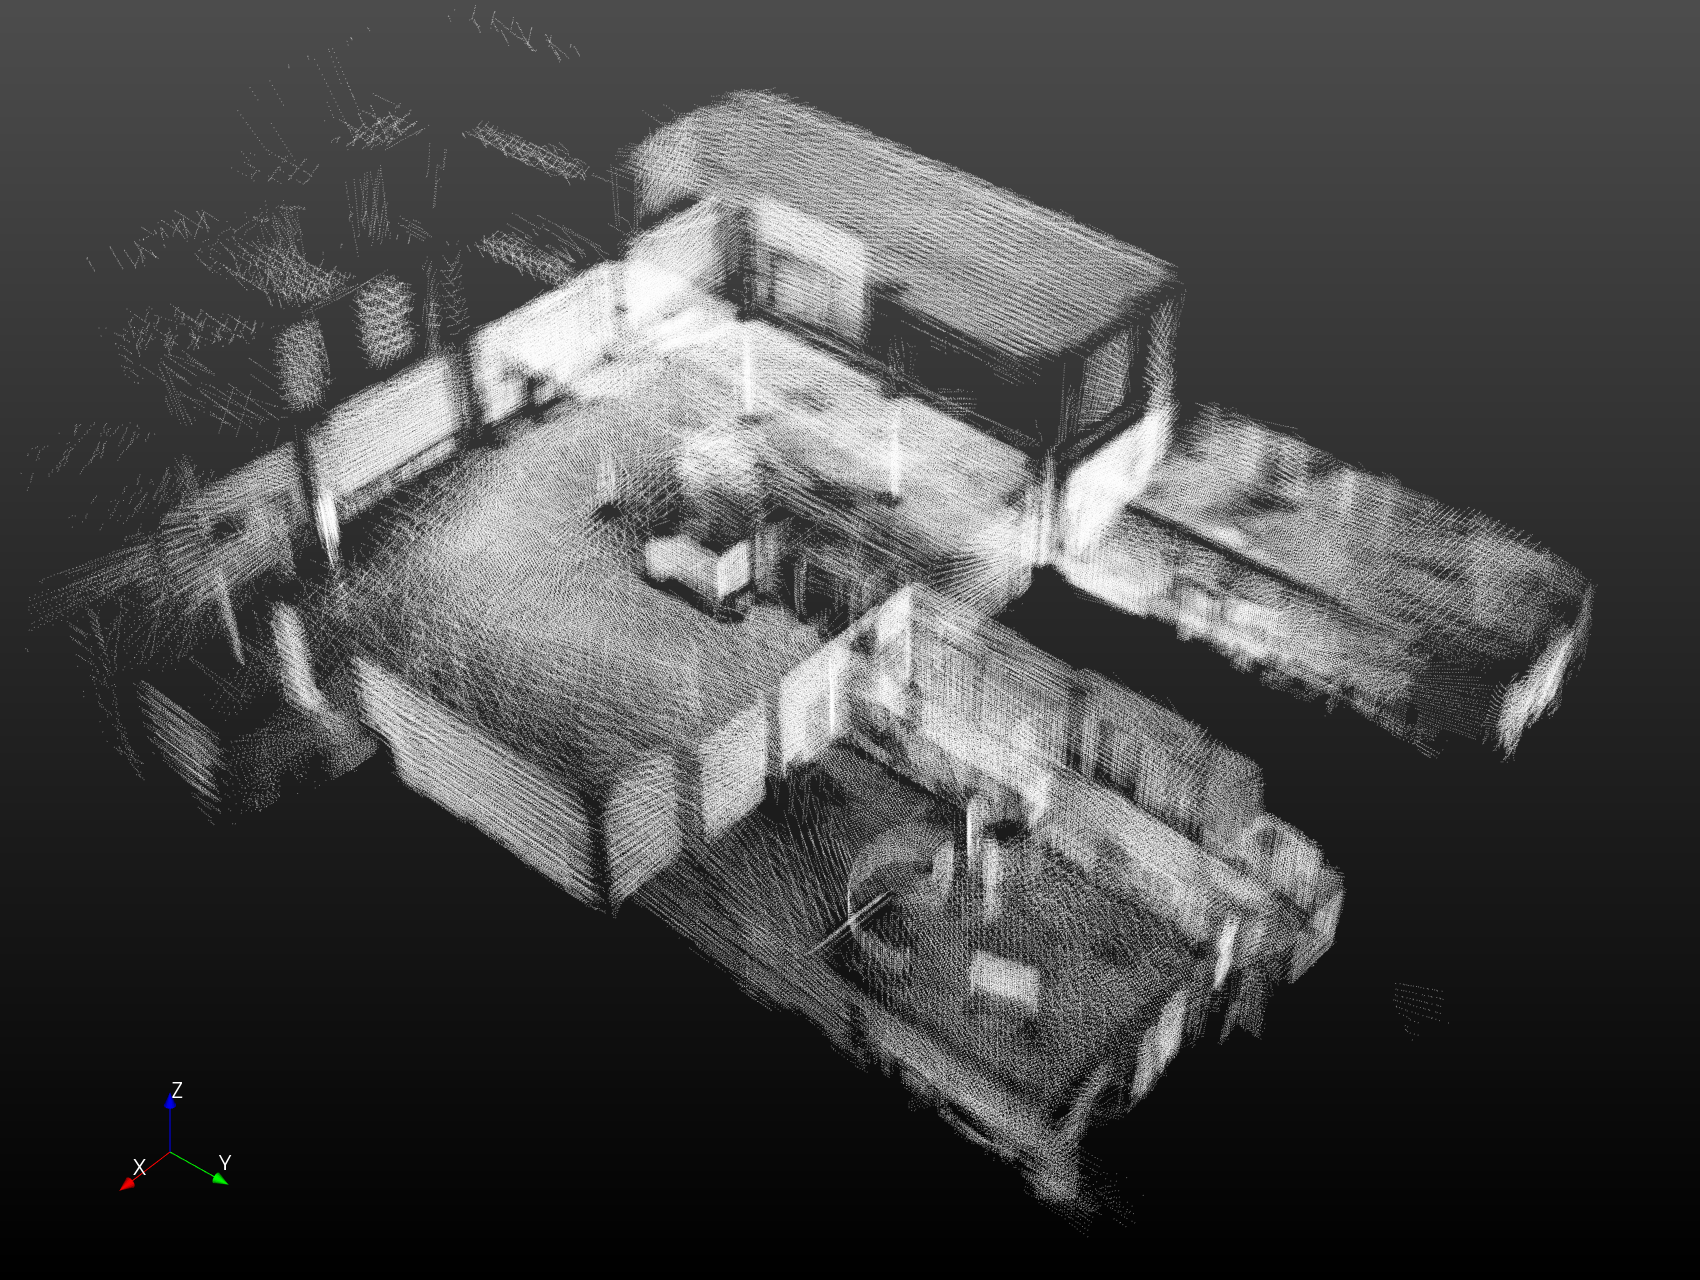
\includegraphics[width = 0.3\linewidth]{PTCL2}} &
		\subfloat{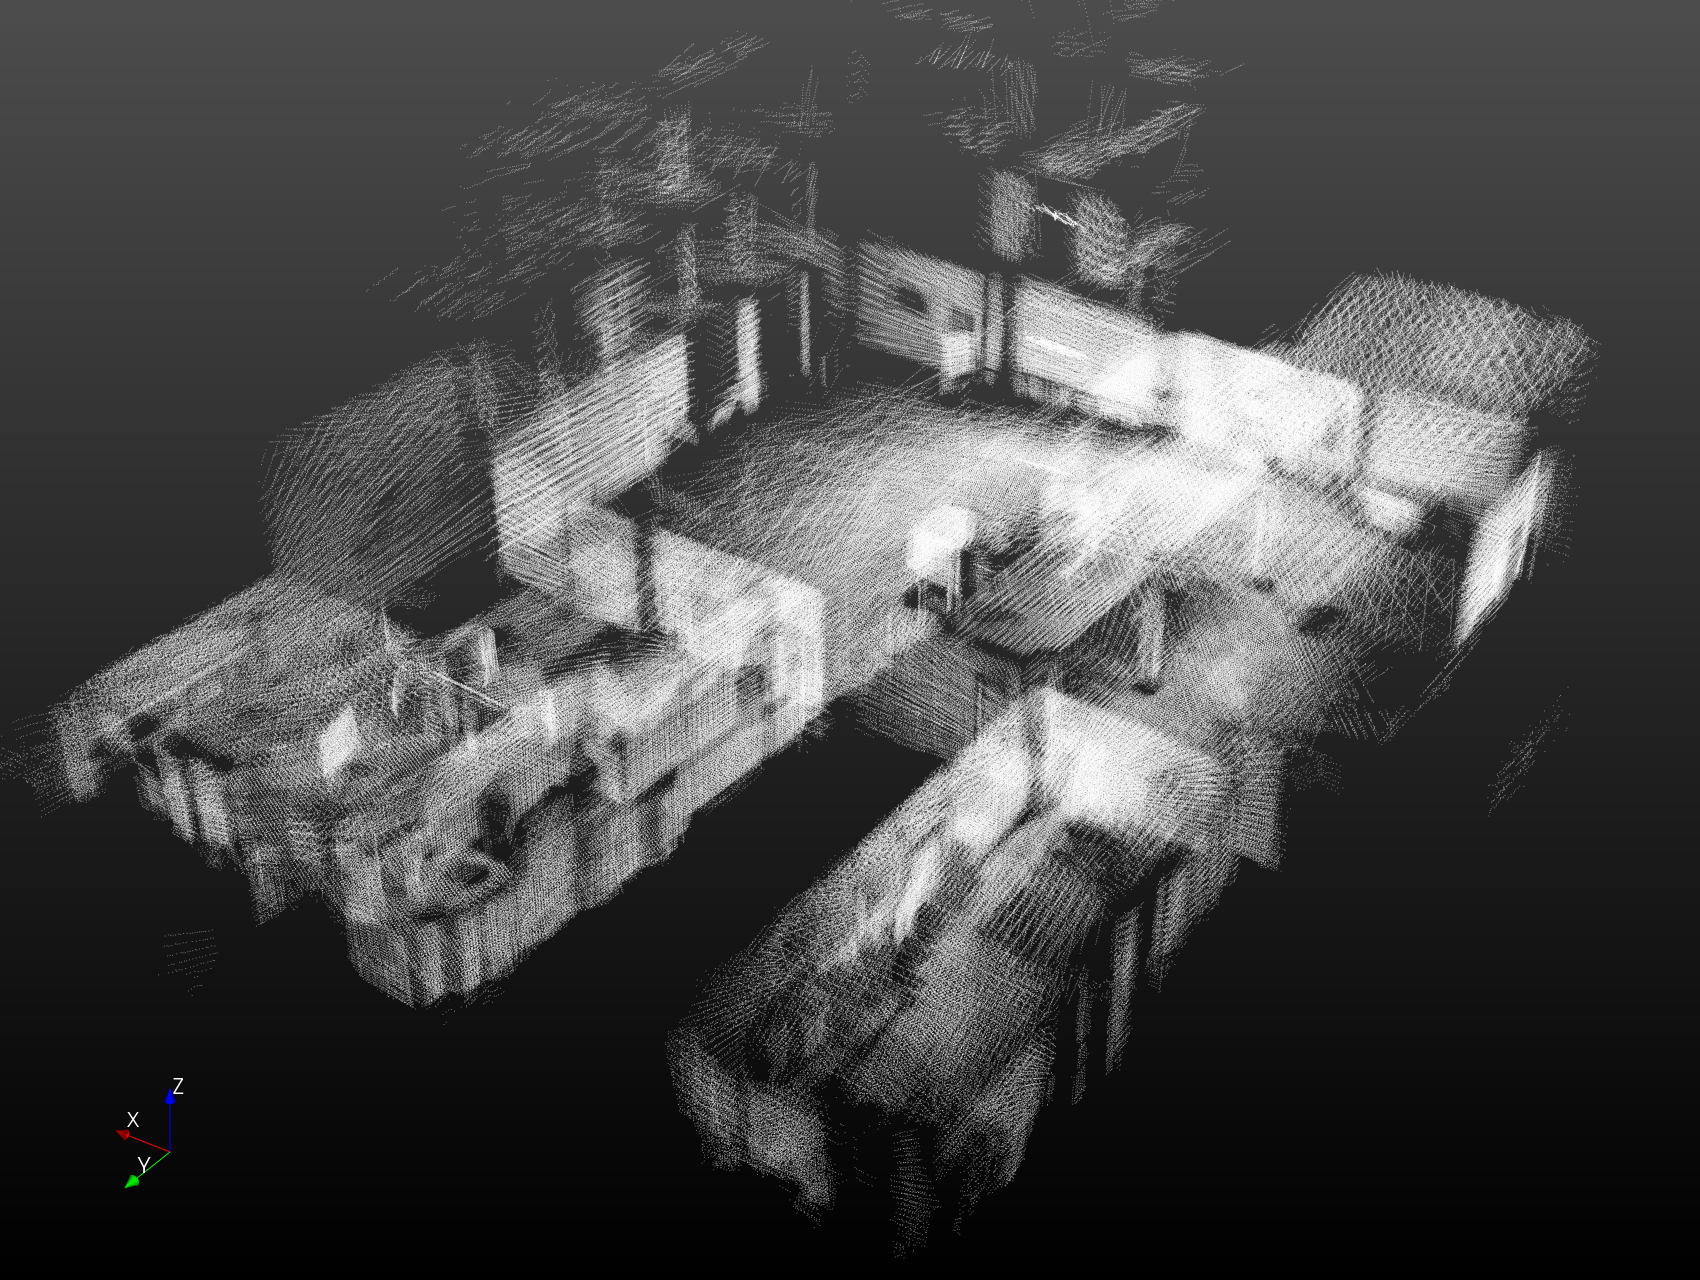
\includegraphics[width = 0.3\linewidth]{PTCL3}} \\
		\subfloat{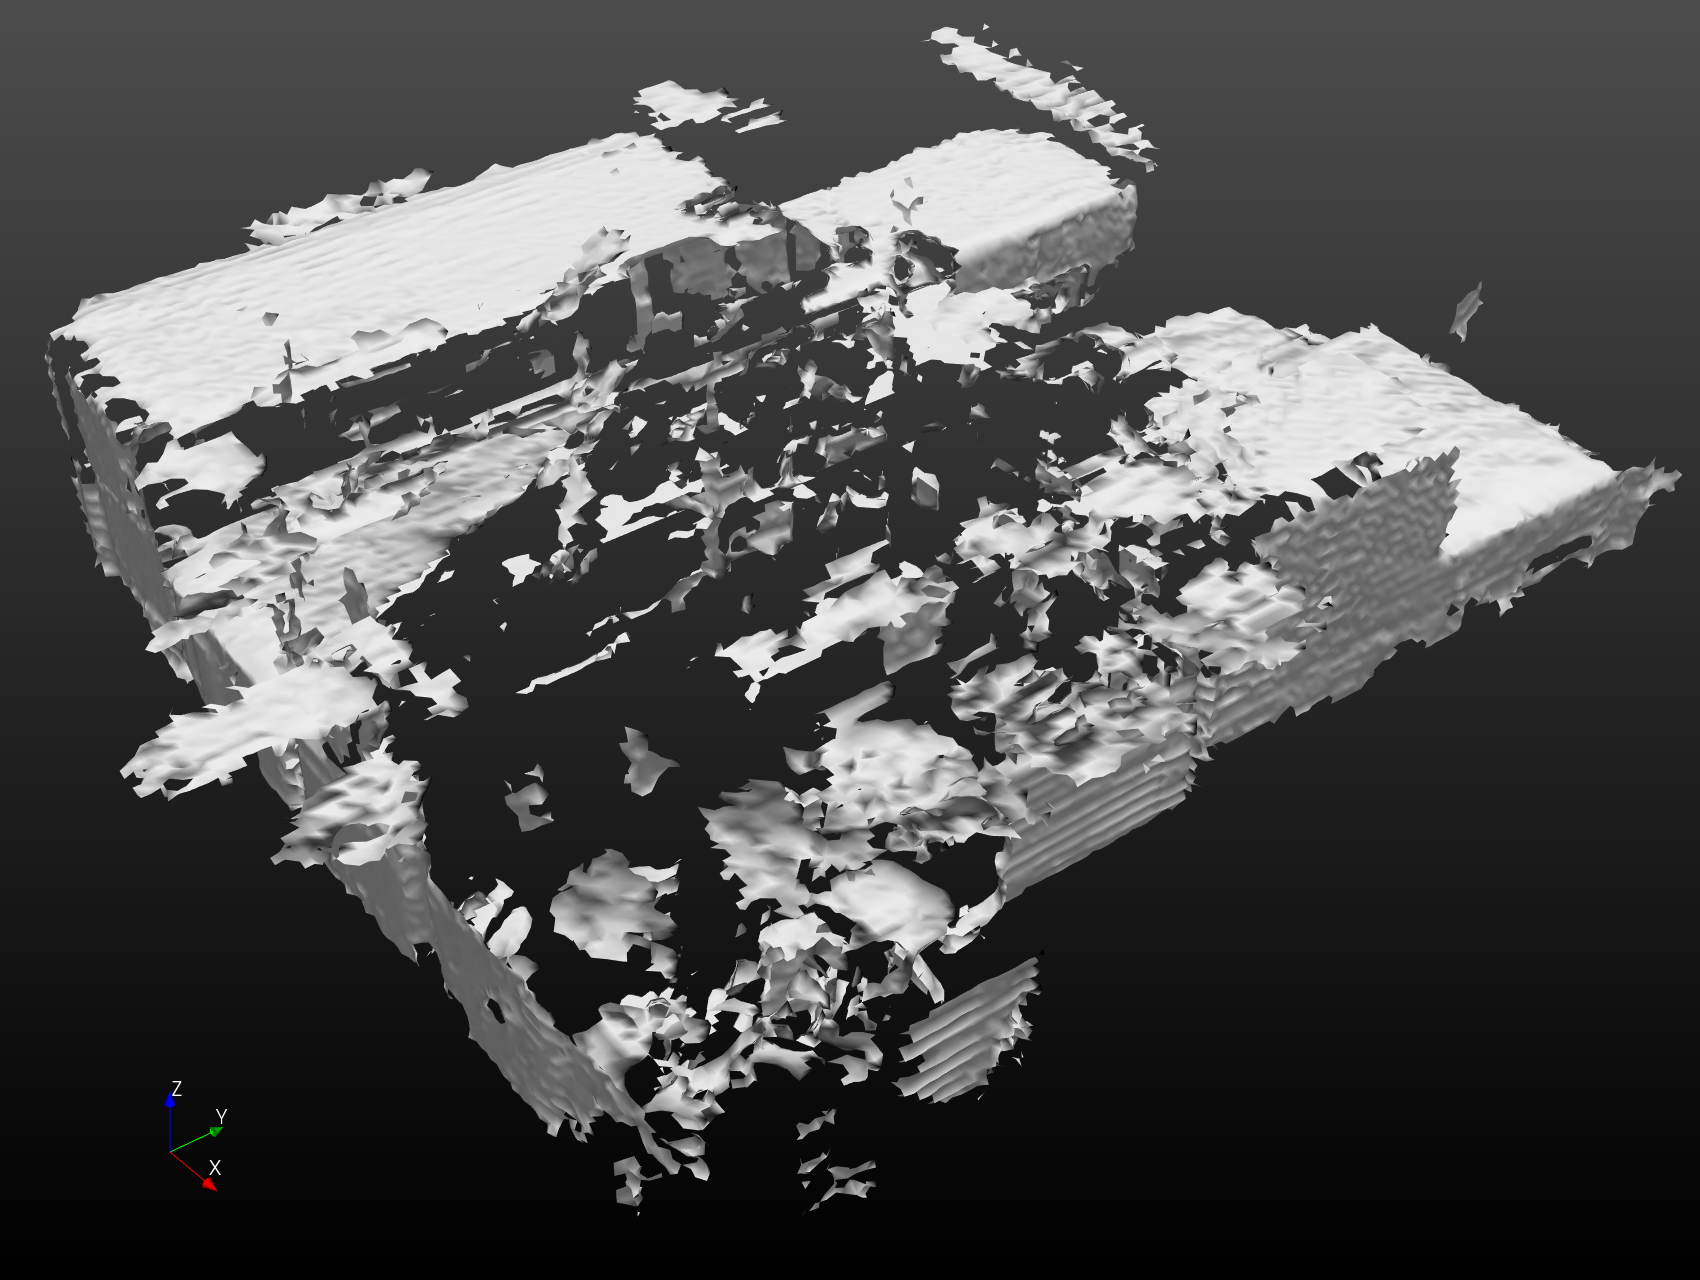
\includegraphics[width = 0.3\linewidth]{Rec1}} &
		\subfloat{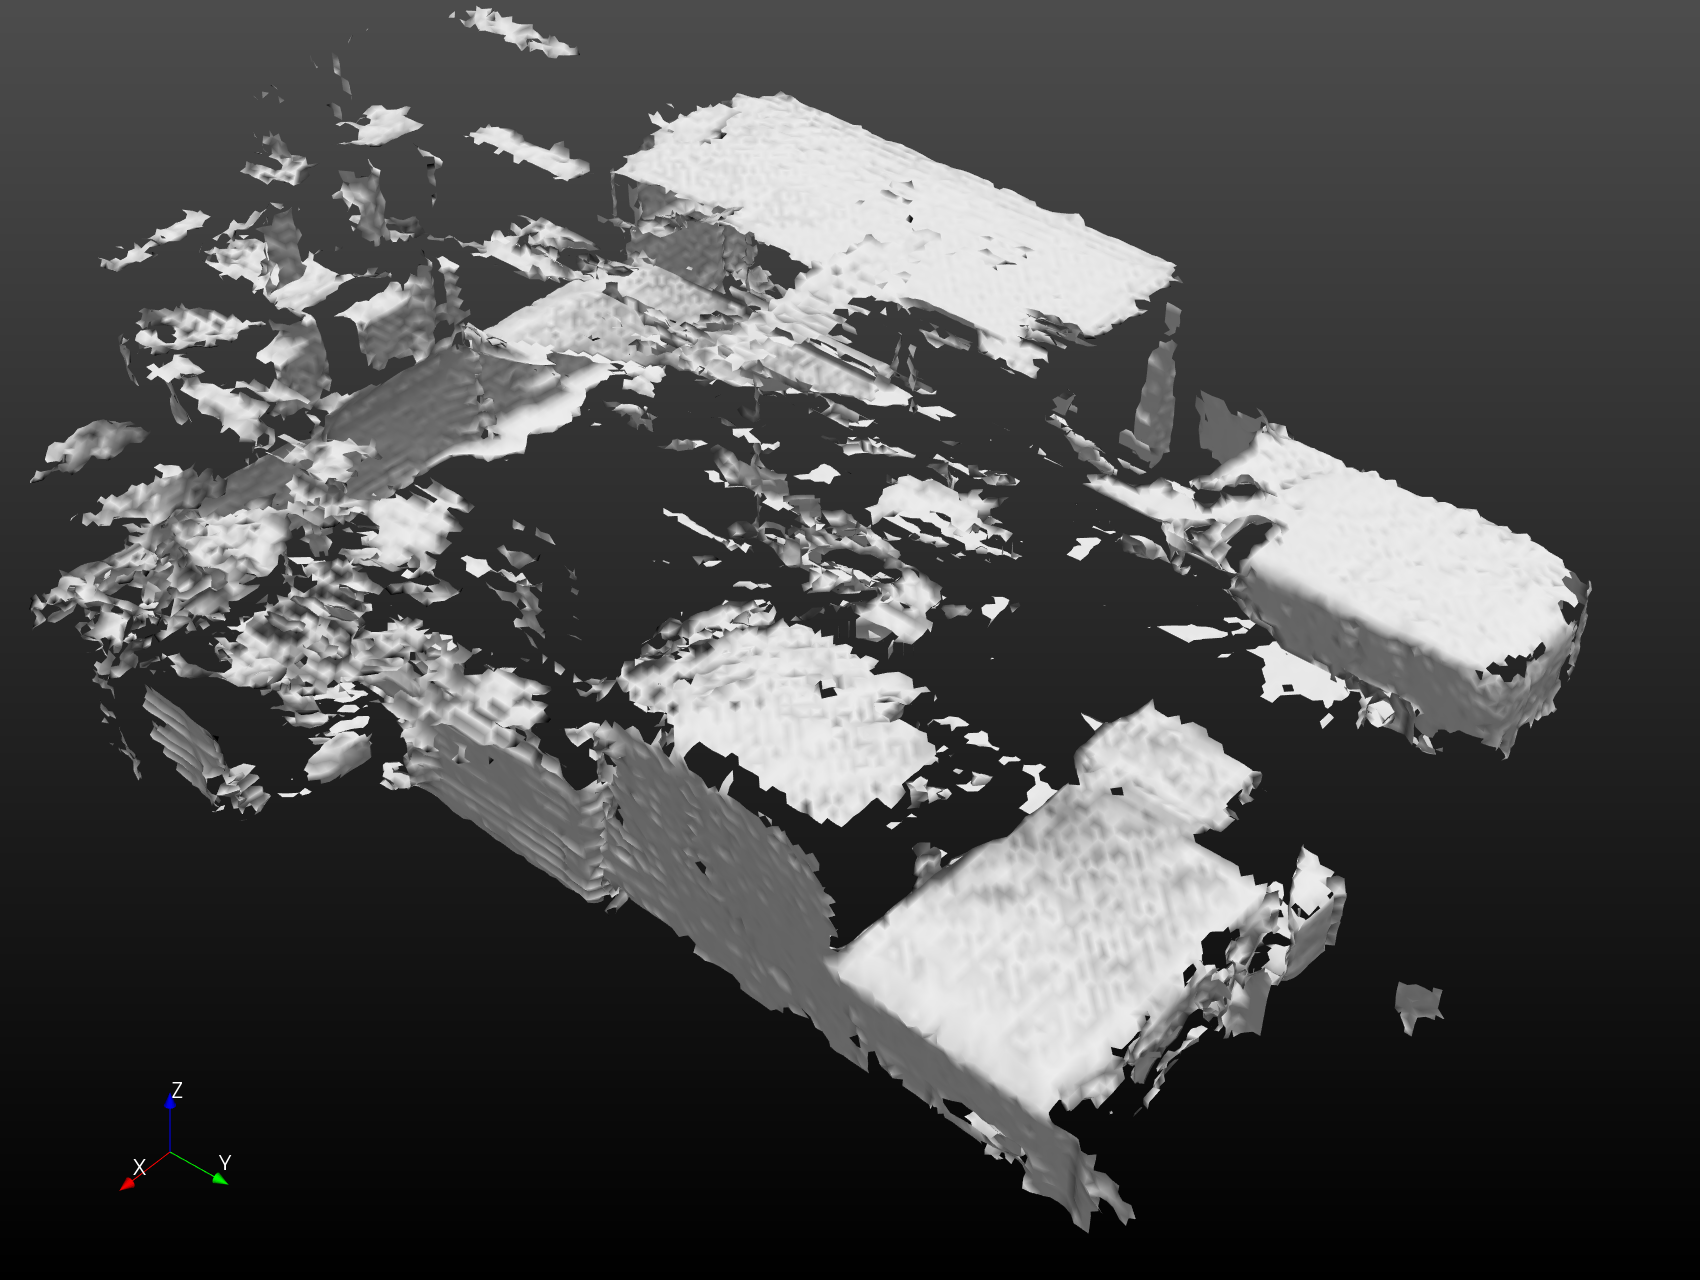
\includegraphics[width = 0.3\linewidth]{Rec2}} &
		\subfloat{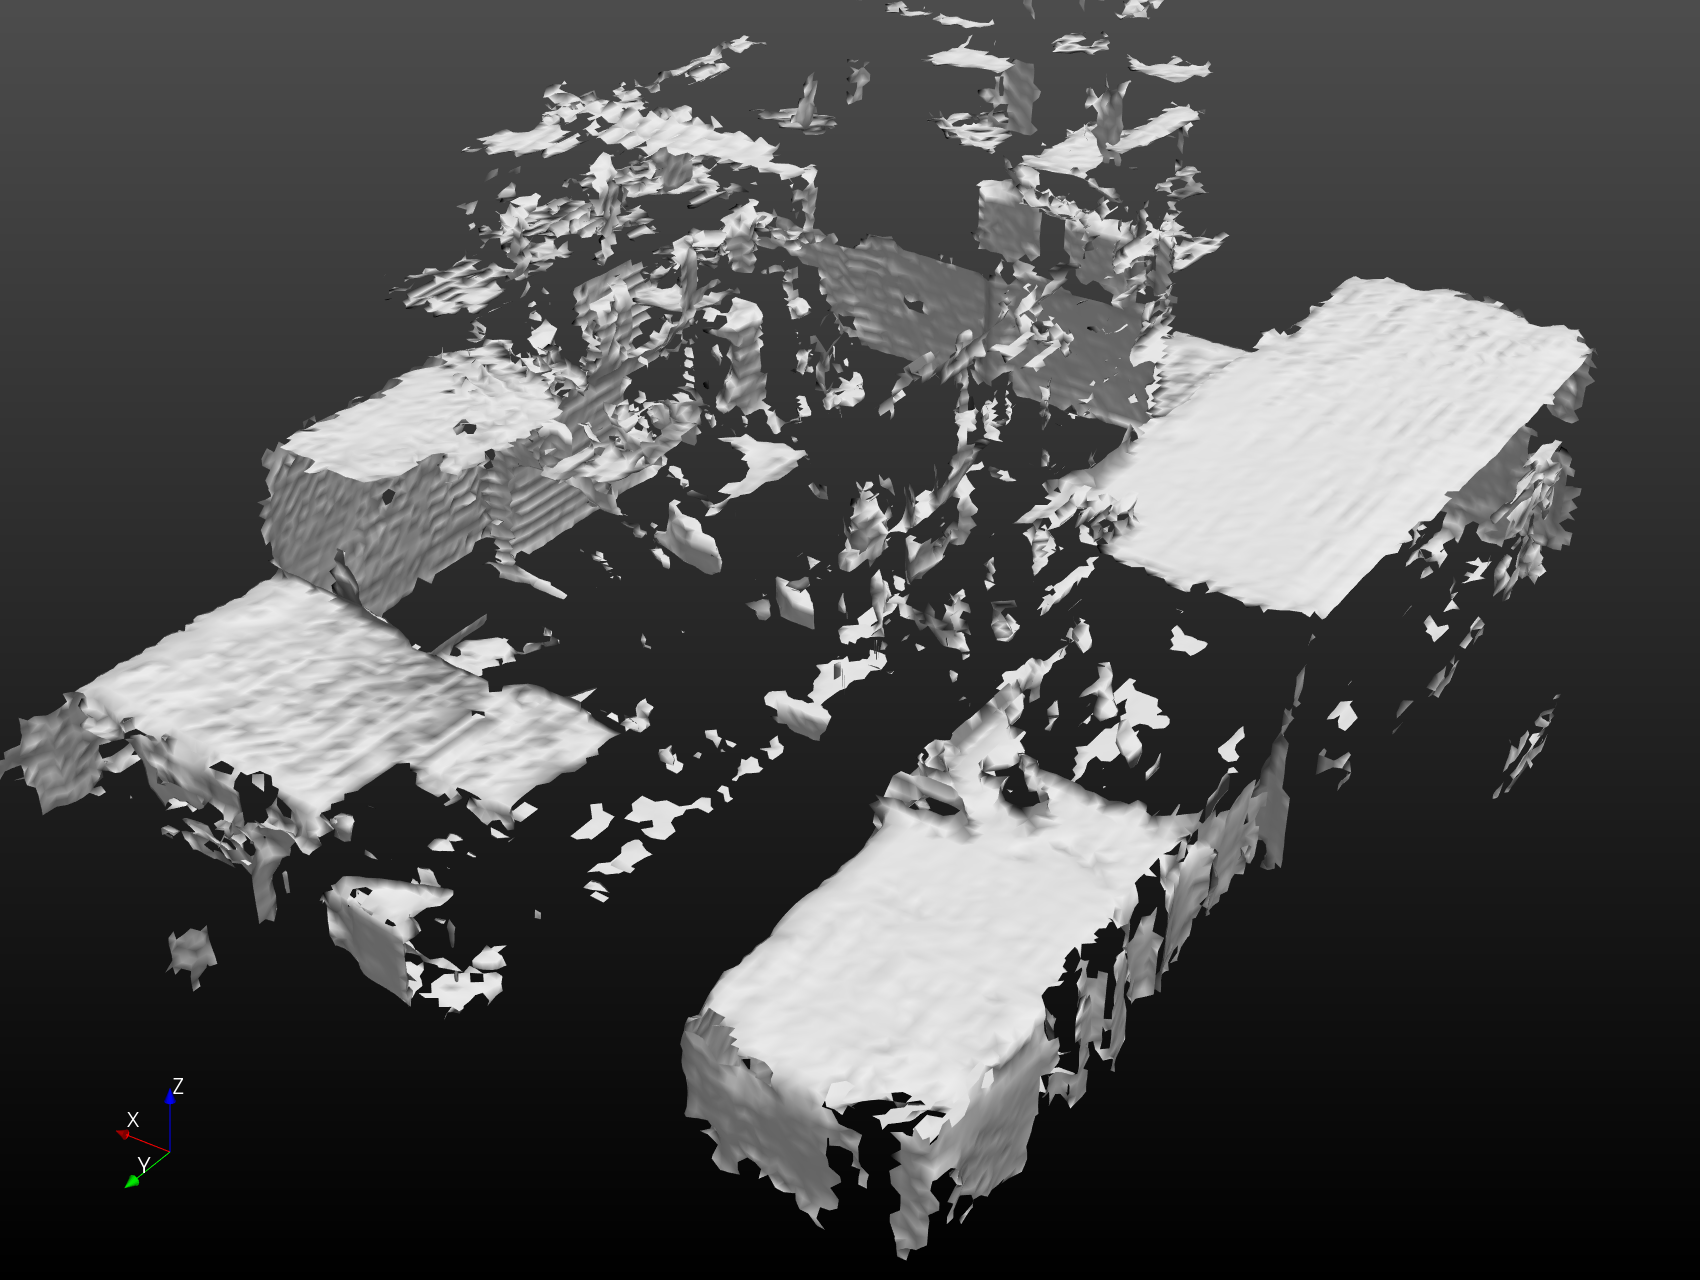
\includegraphics[width = 0.3\linewidth]{Rec3}} \\
		\subfloat{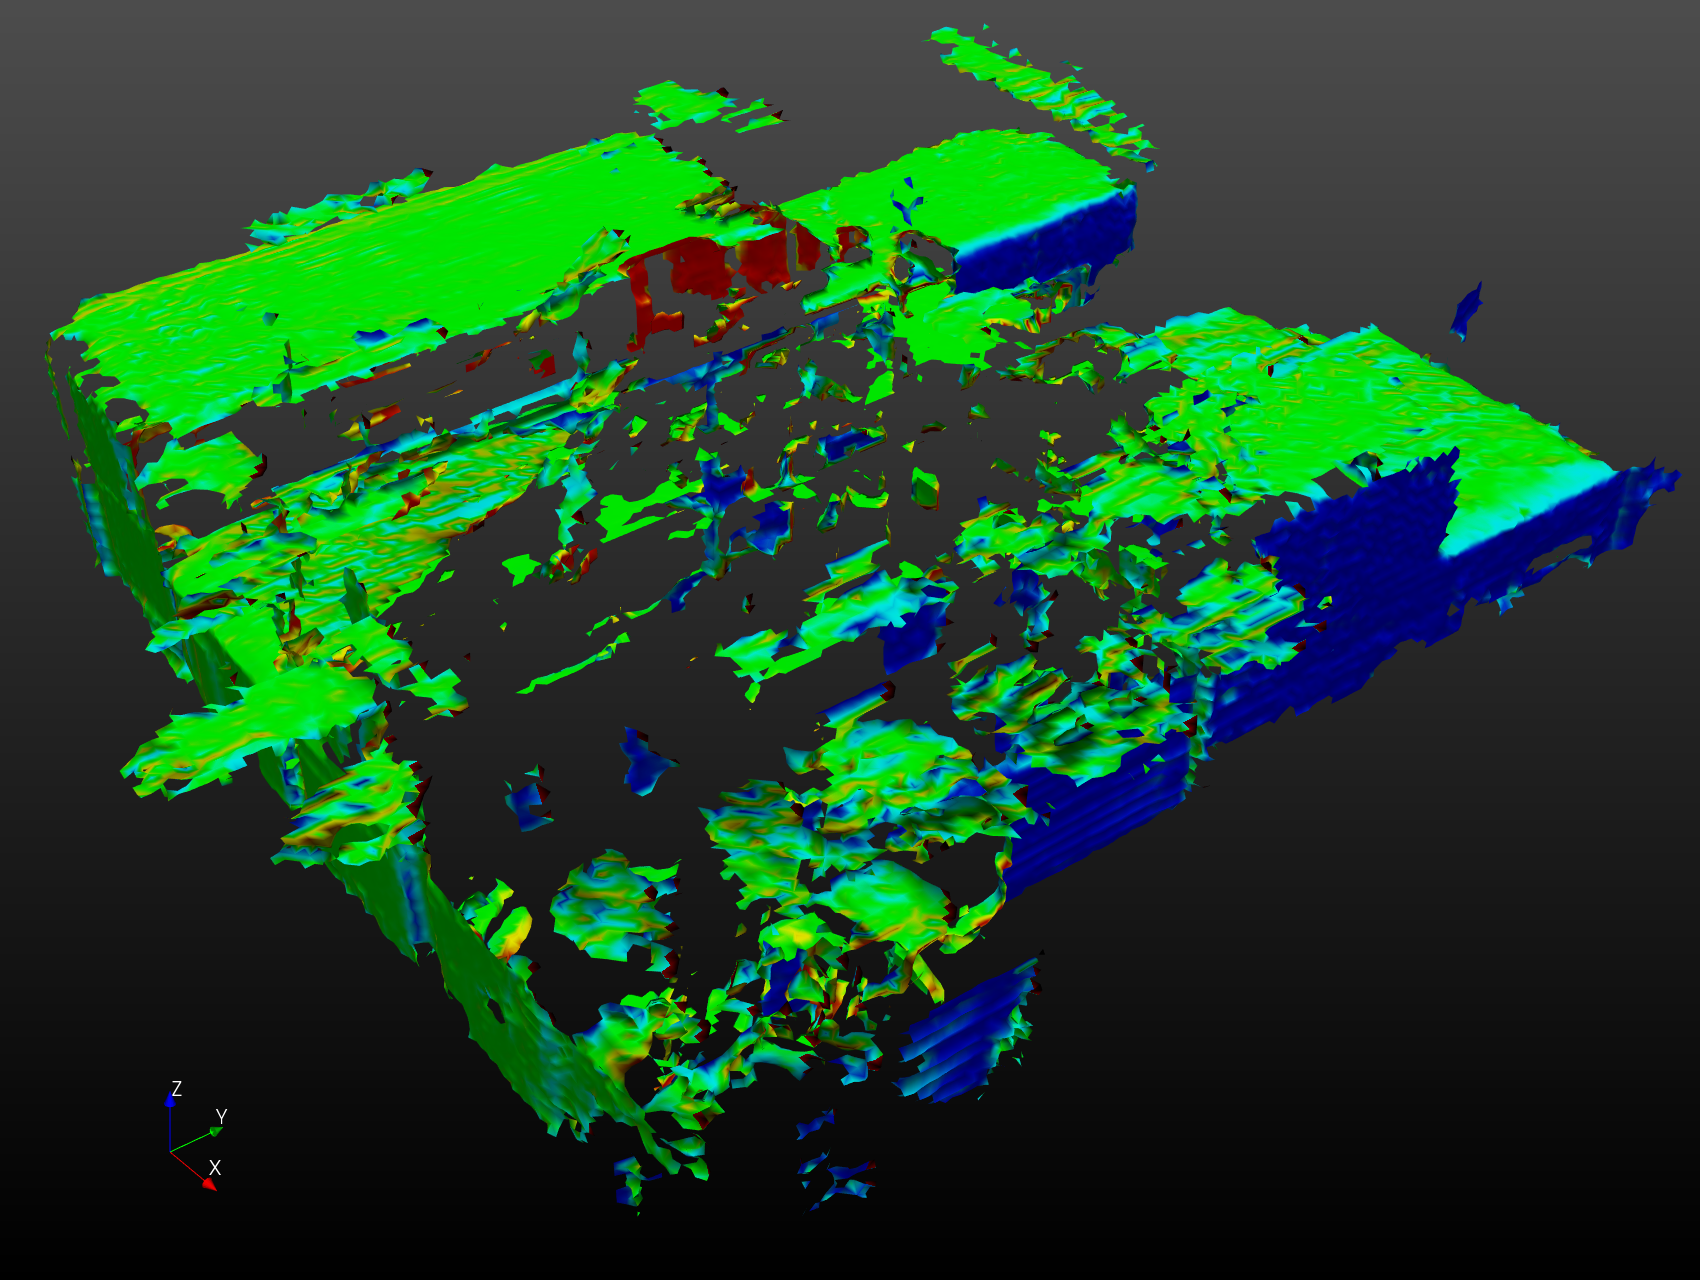
\includegraphics[width = 0.3\linewidth]{Rec1N}} &
		\subfloat{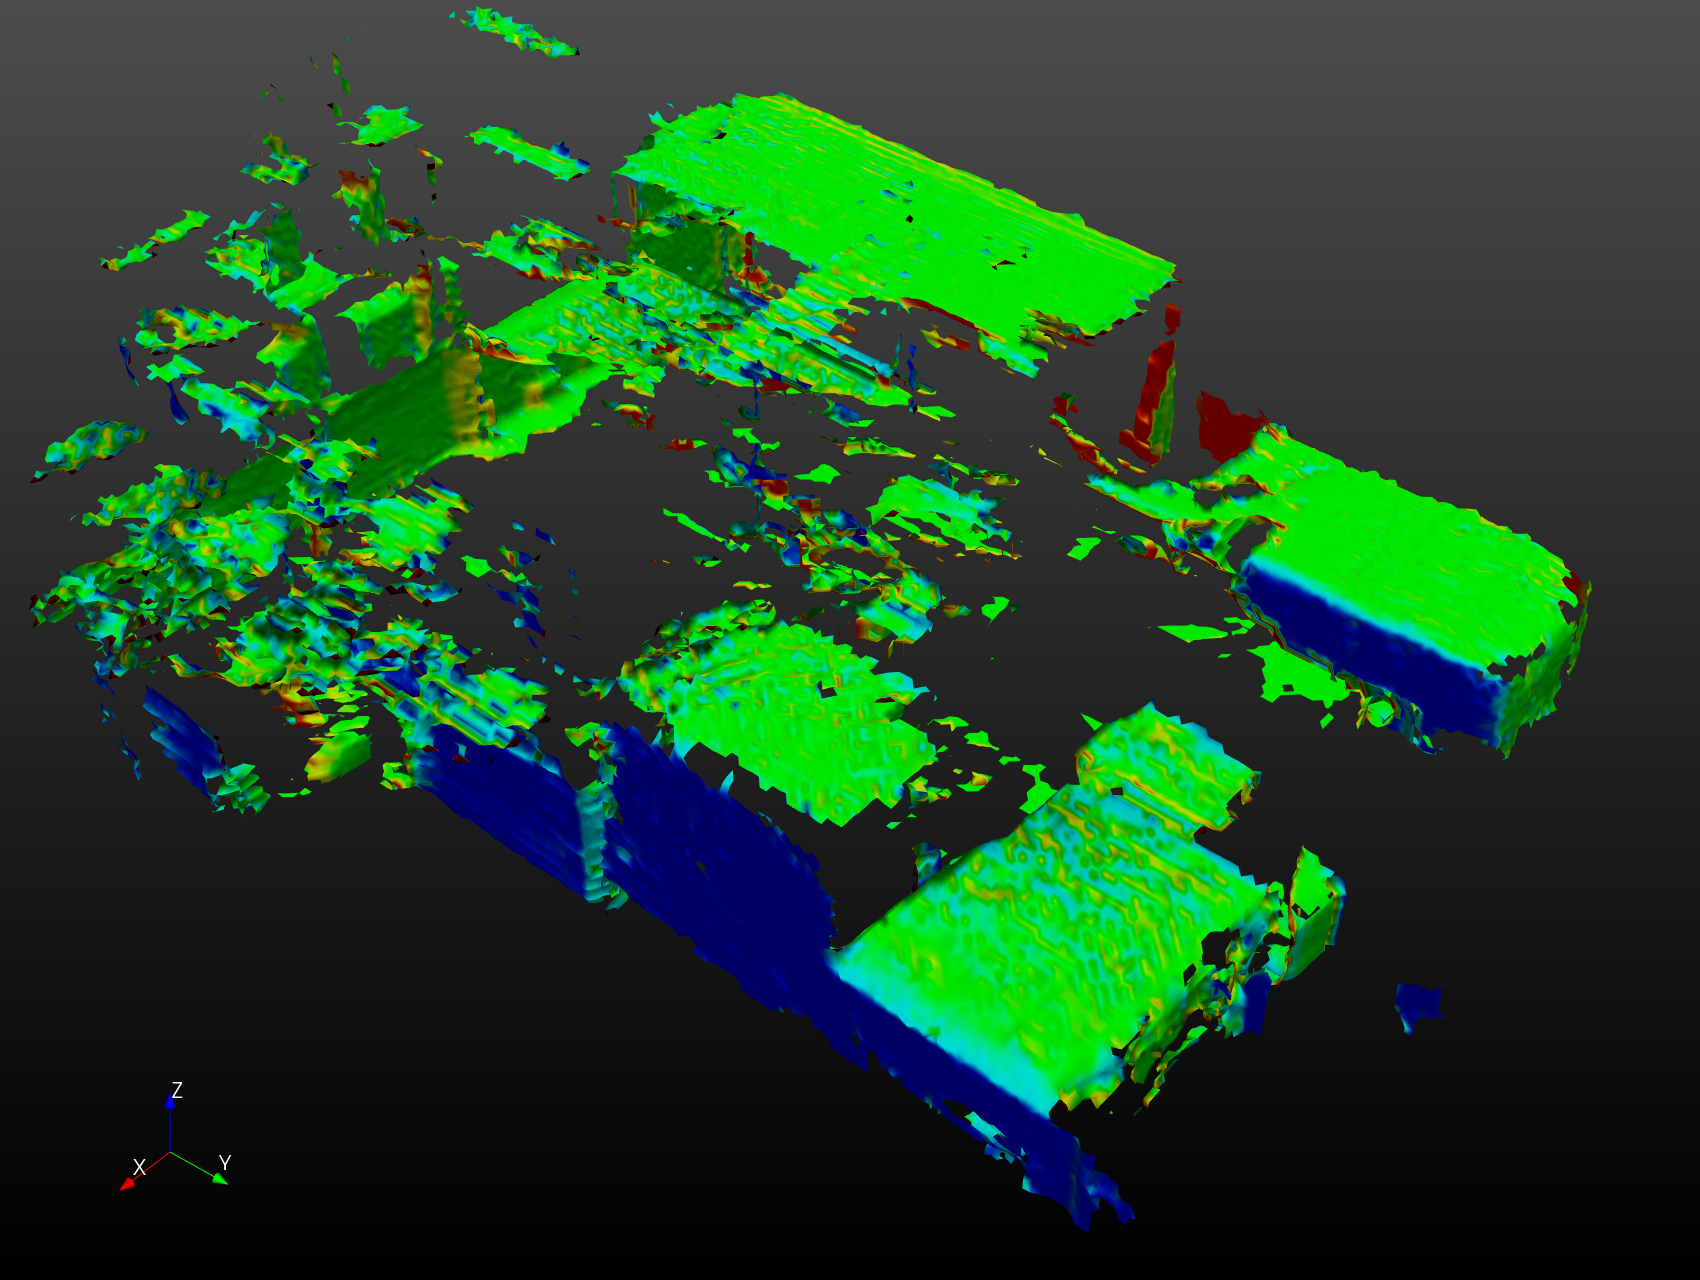
\includegraphics[width = 0.3\linewidth]{Rec2N}} &
		\subfloat{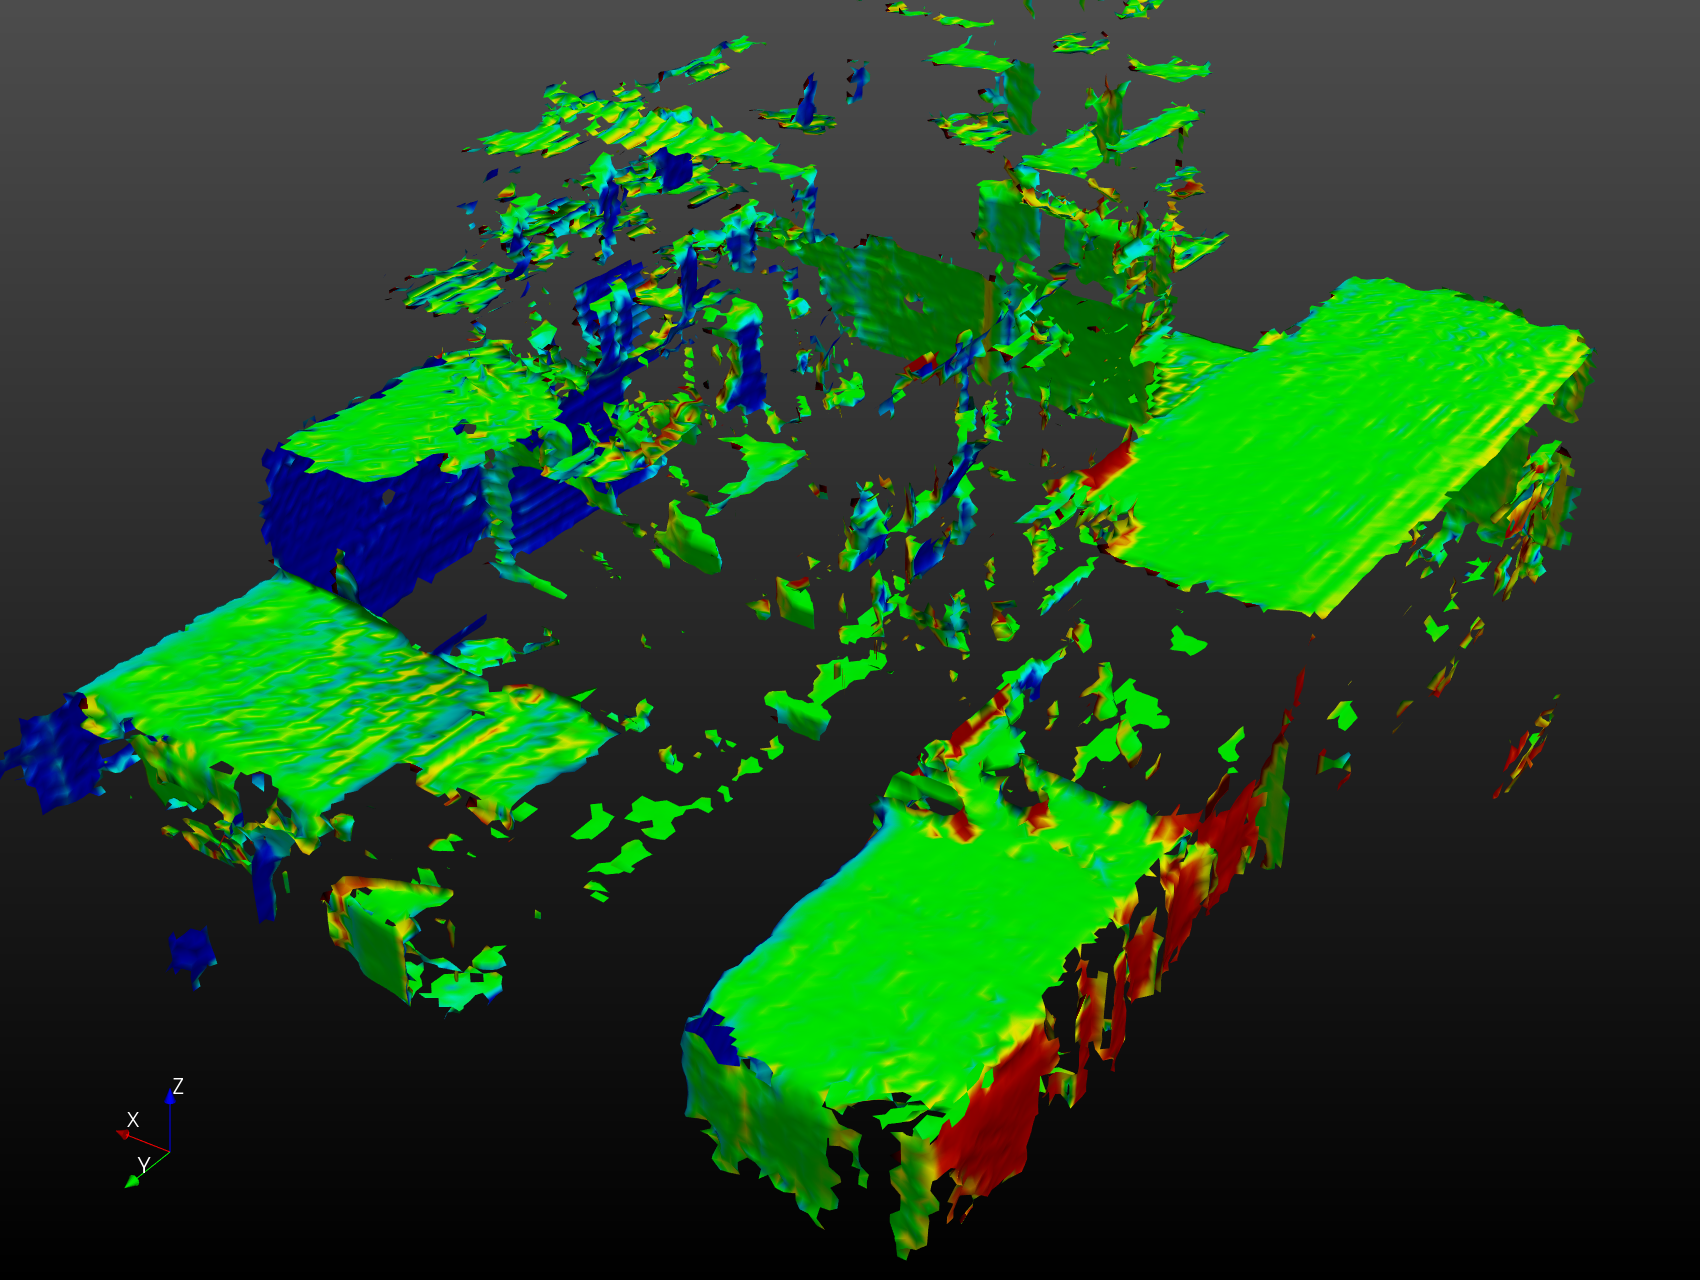
\includegraphics[width = 0.3\linewidth]{Rec3N}} \\
		\subfloat{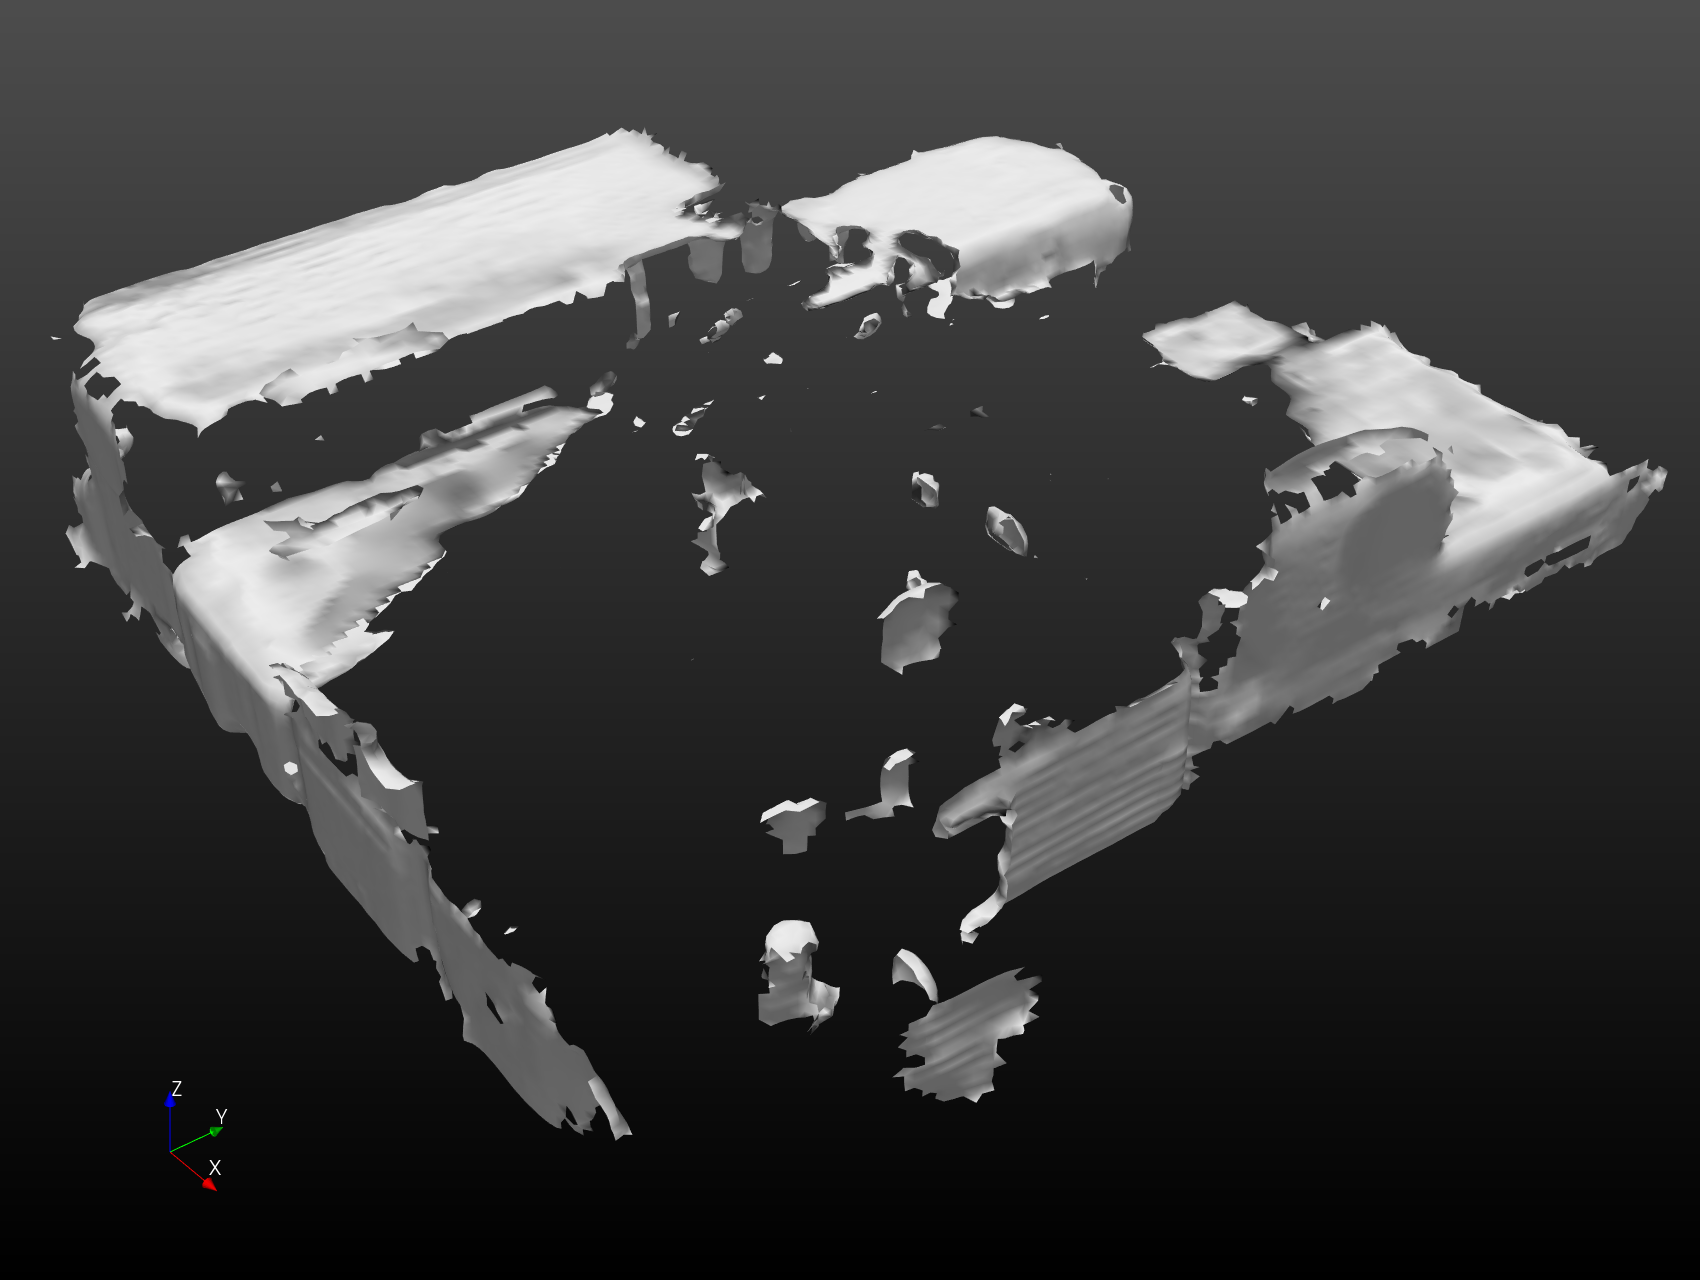
\includegraphics[width = 0.3\linewidth]{RegRec1}} &
		\subfloat{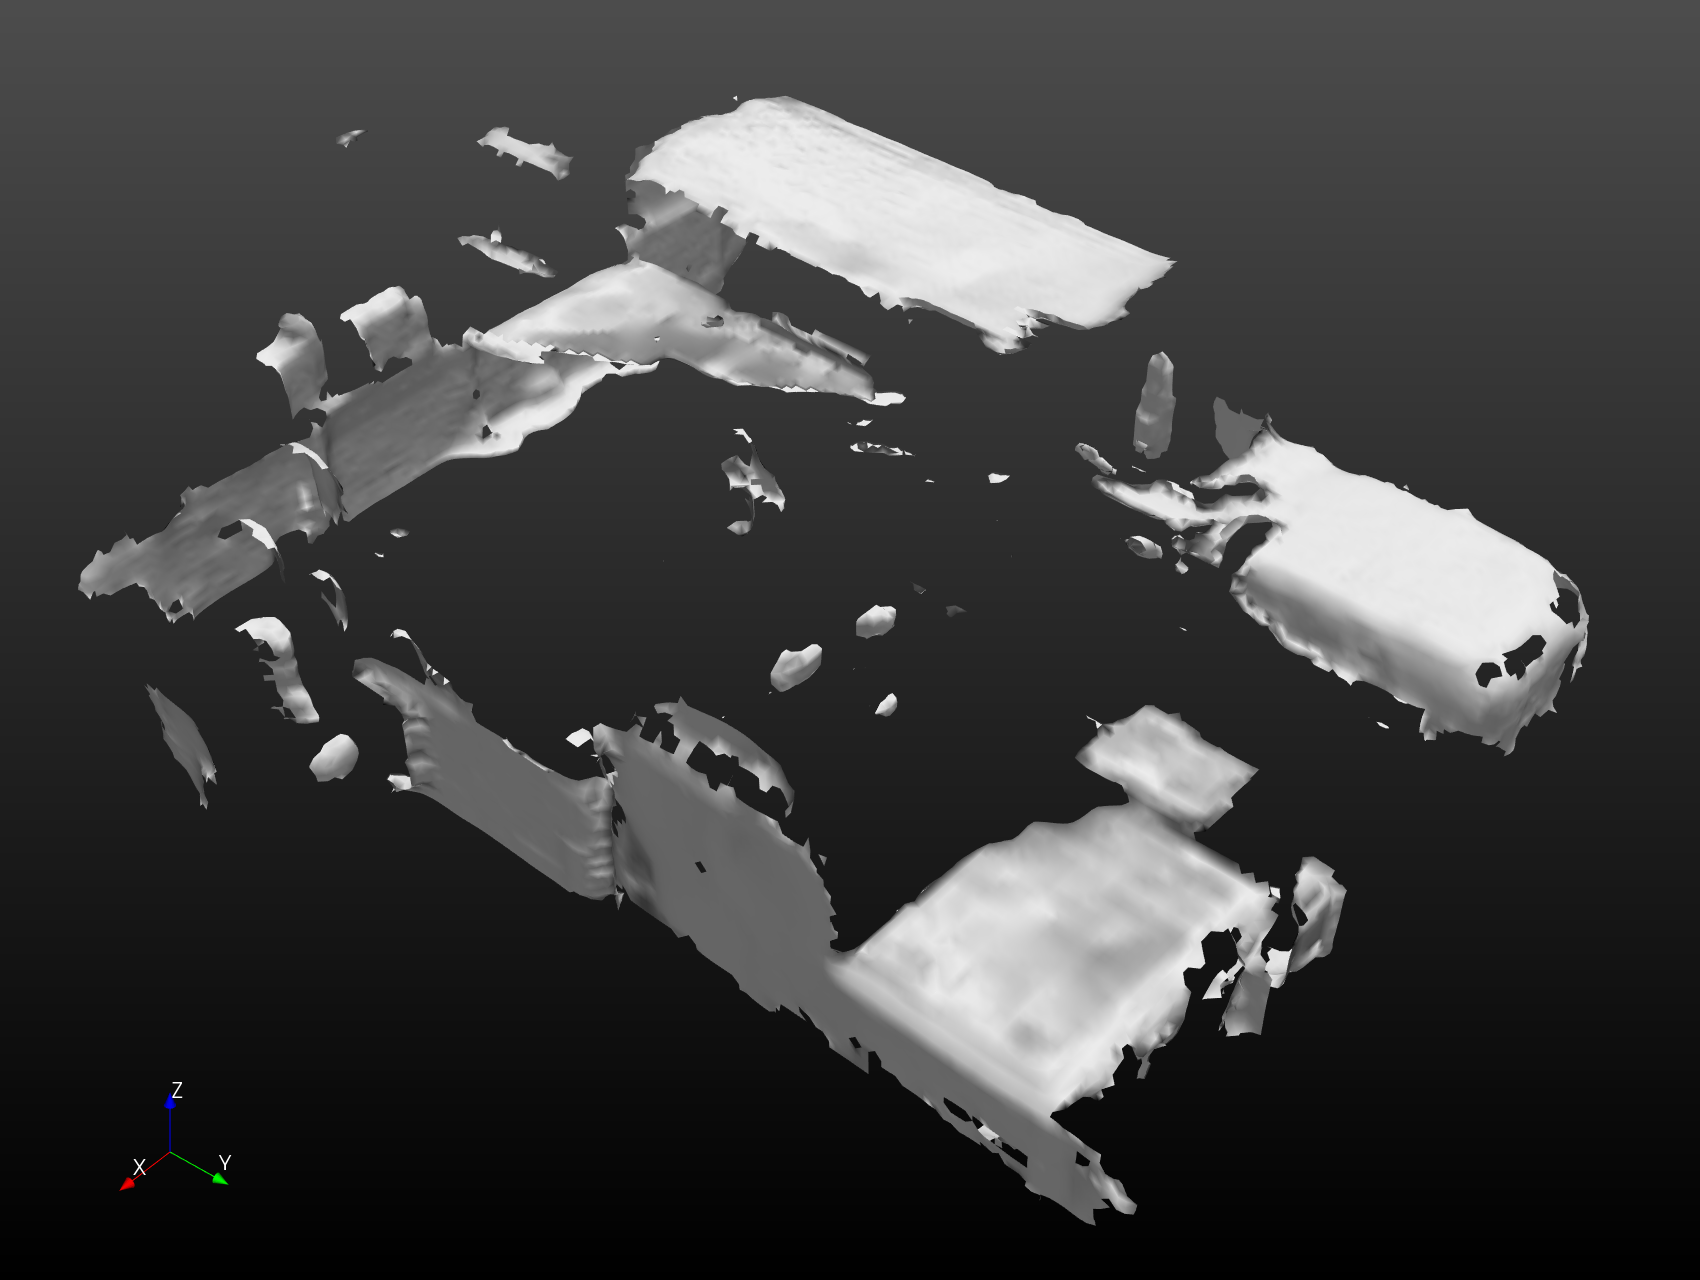
\includegraphics[width = 0.3\linewidth]{RegRec2}} &
		\subfloat{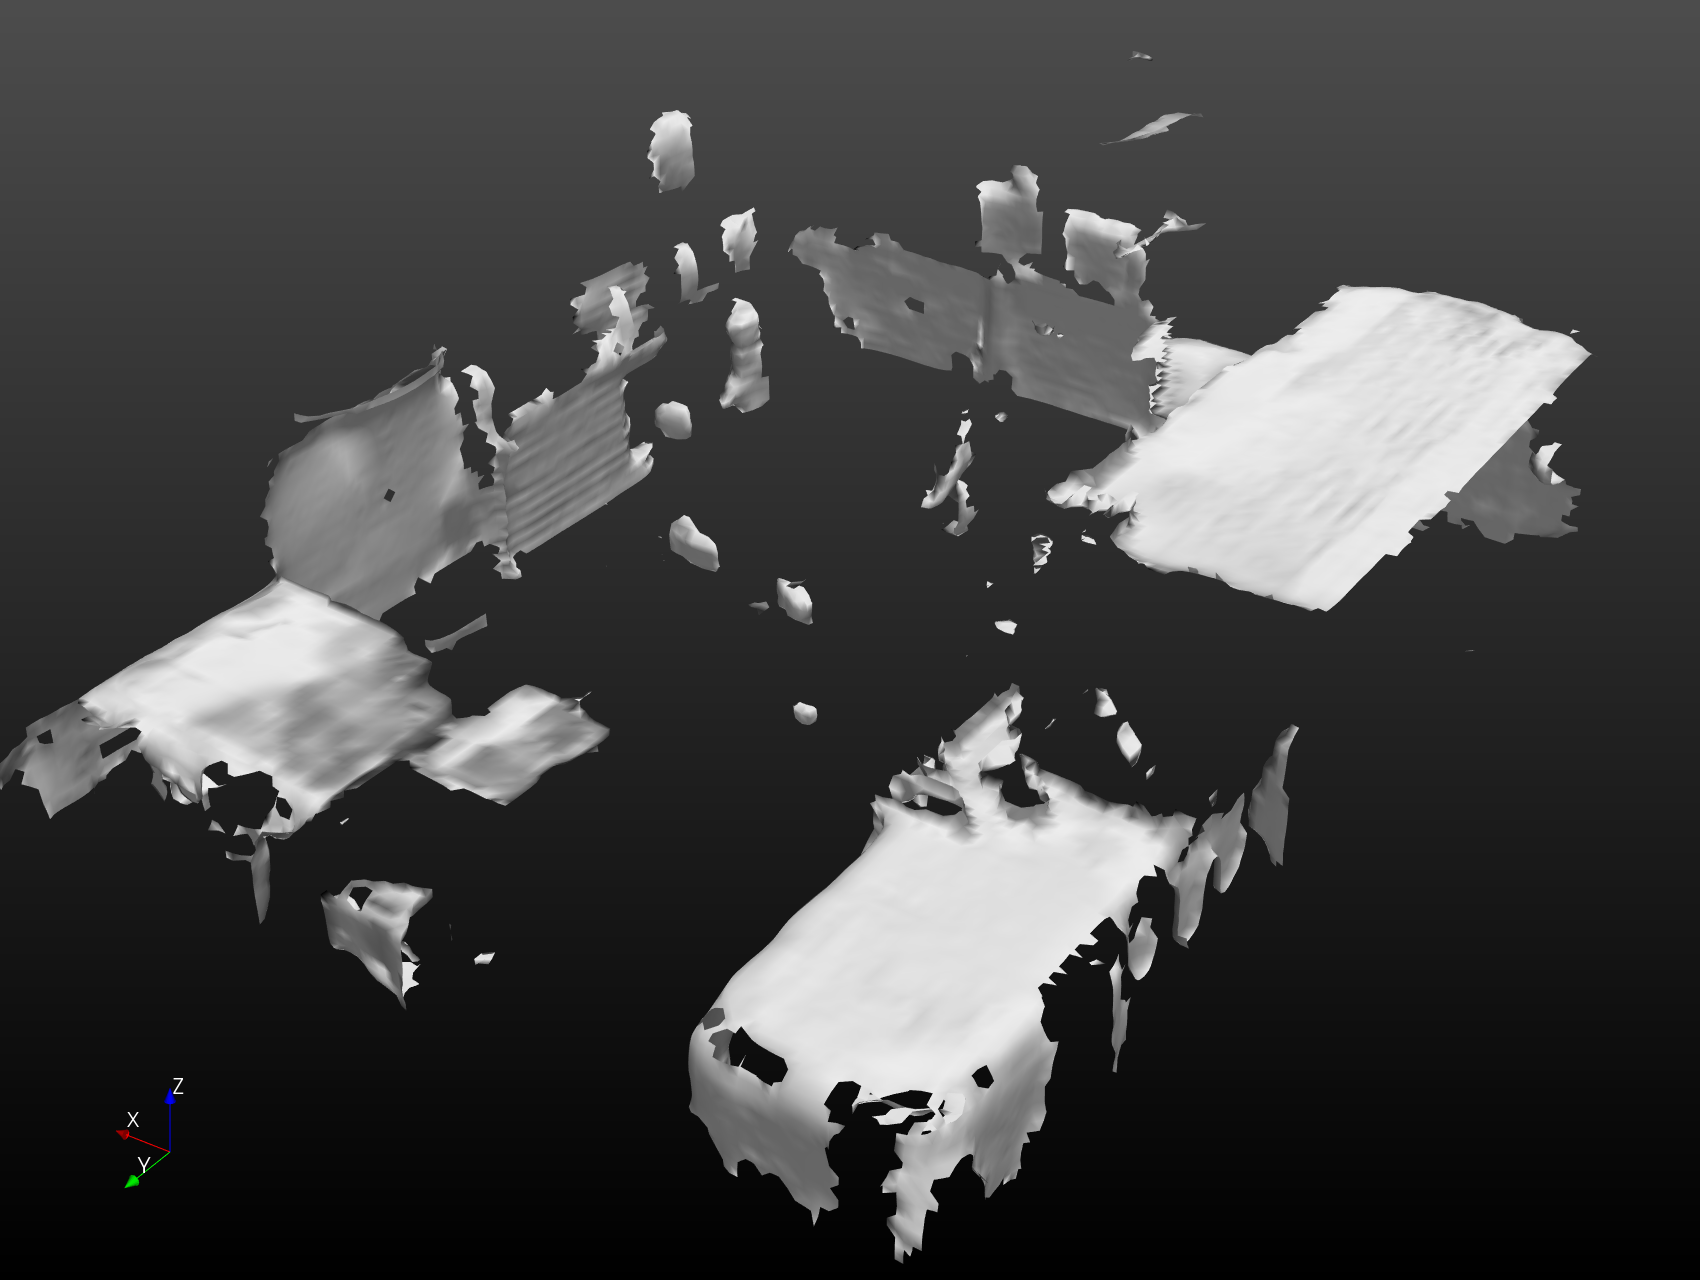
\includegraphics[width = 0.3\linewidth]{RegRec3}}\\
		\subfloat{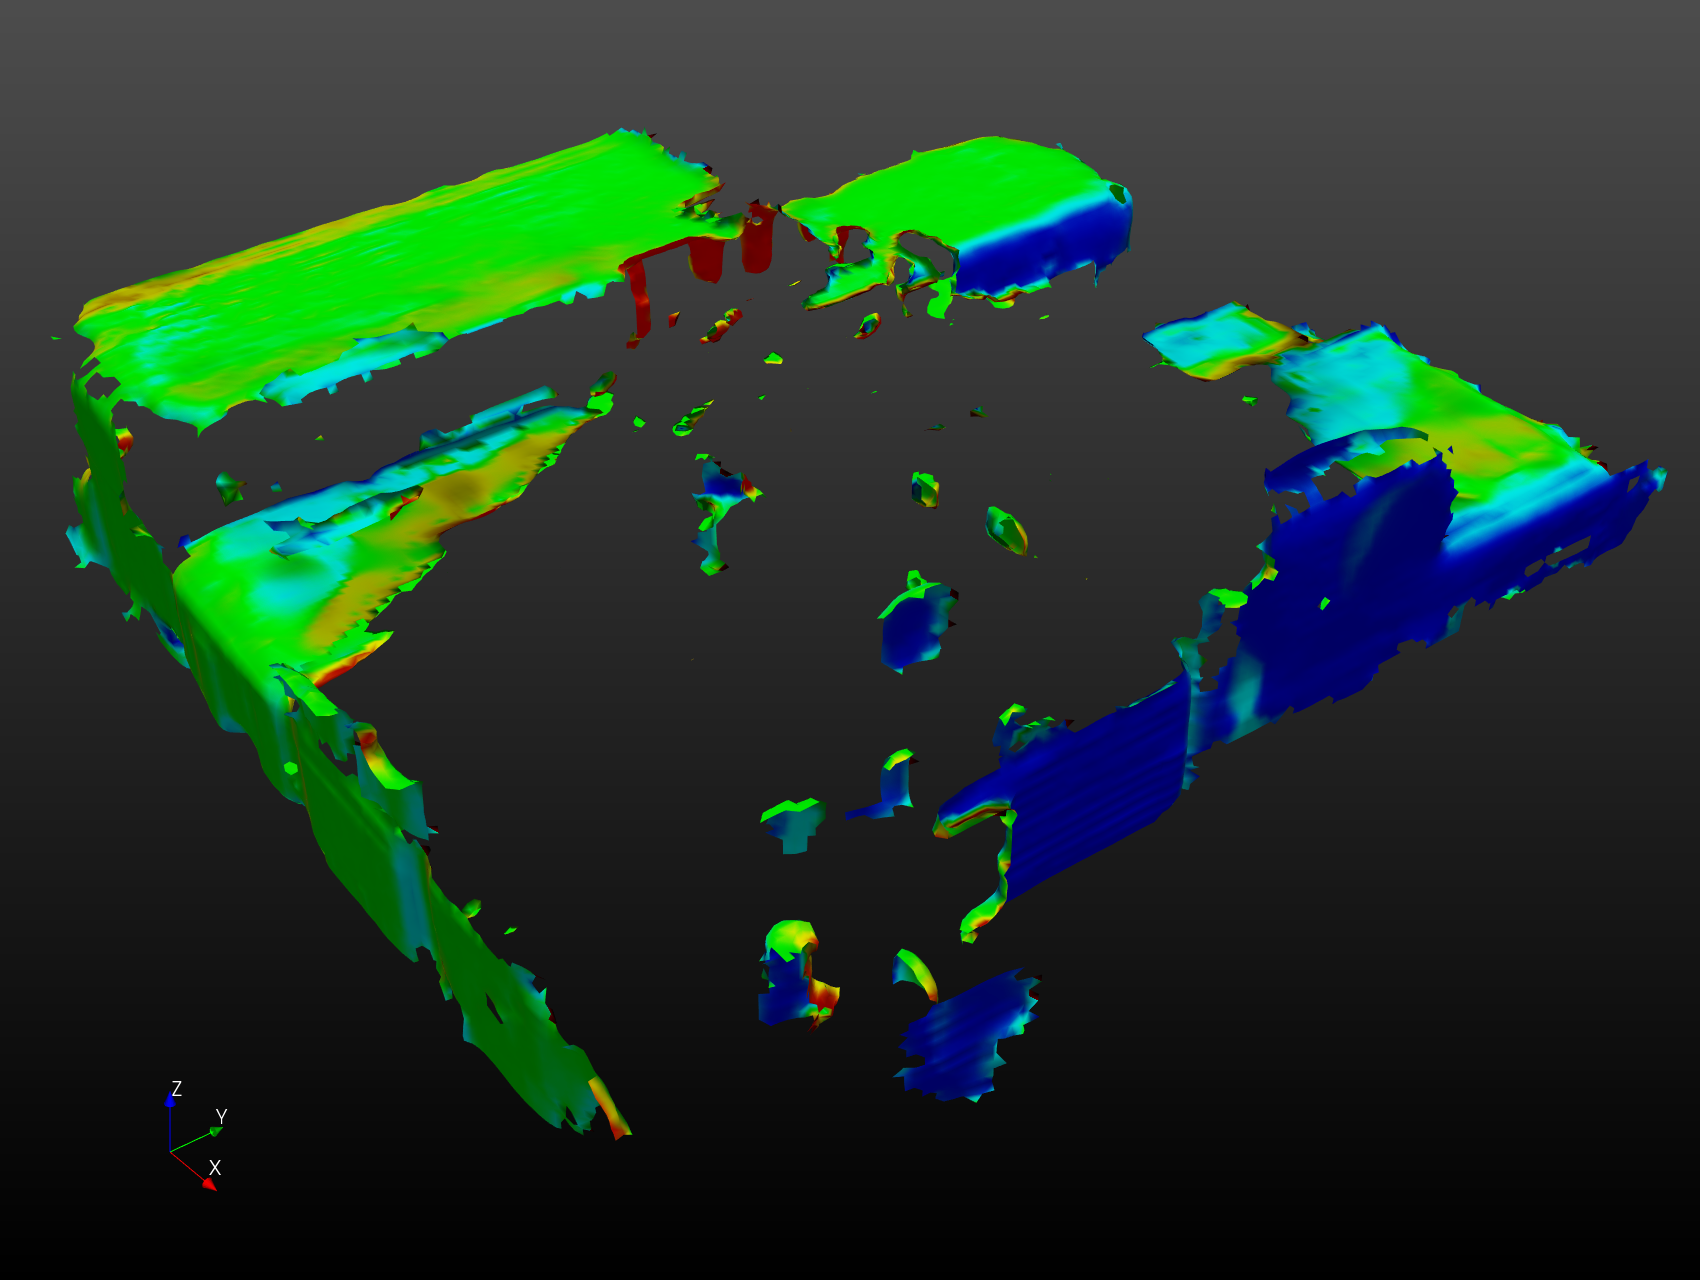
\includegraphics[width = 0.3\linewidth]{RegRec1N}} &
		\subfloat{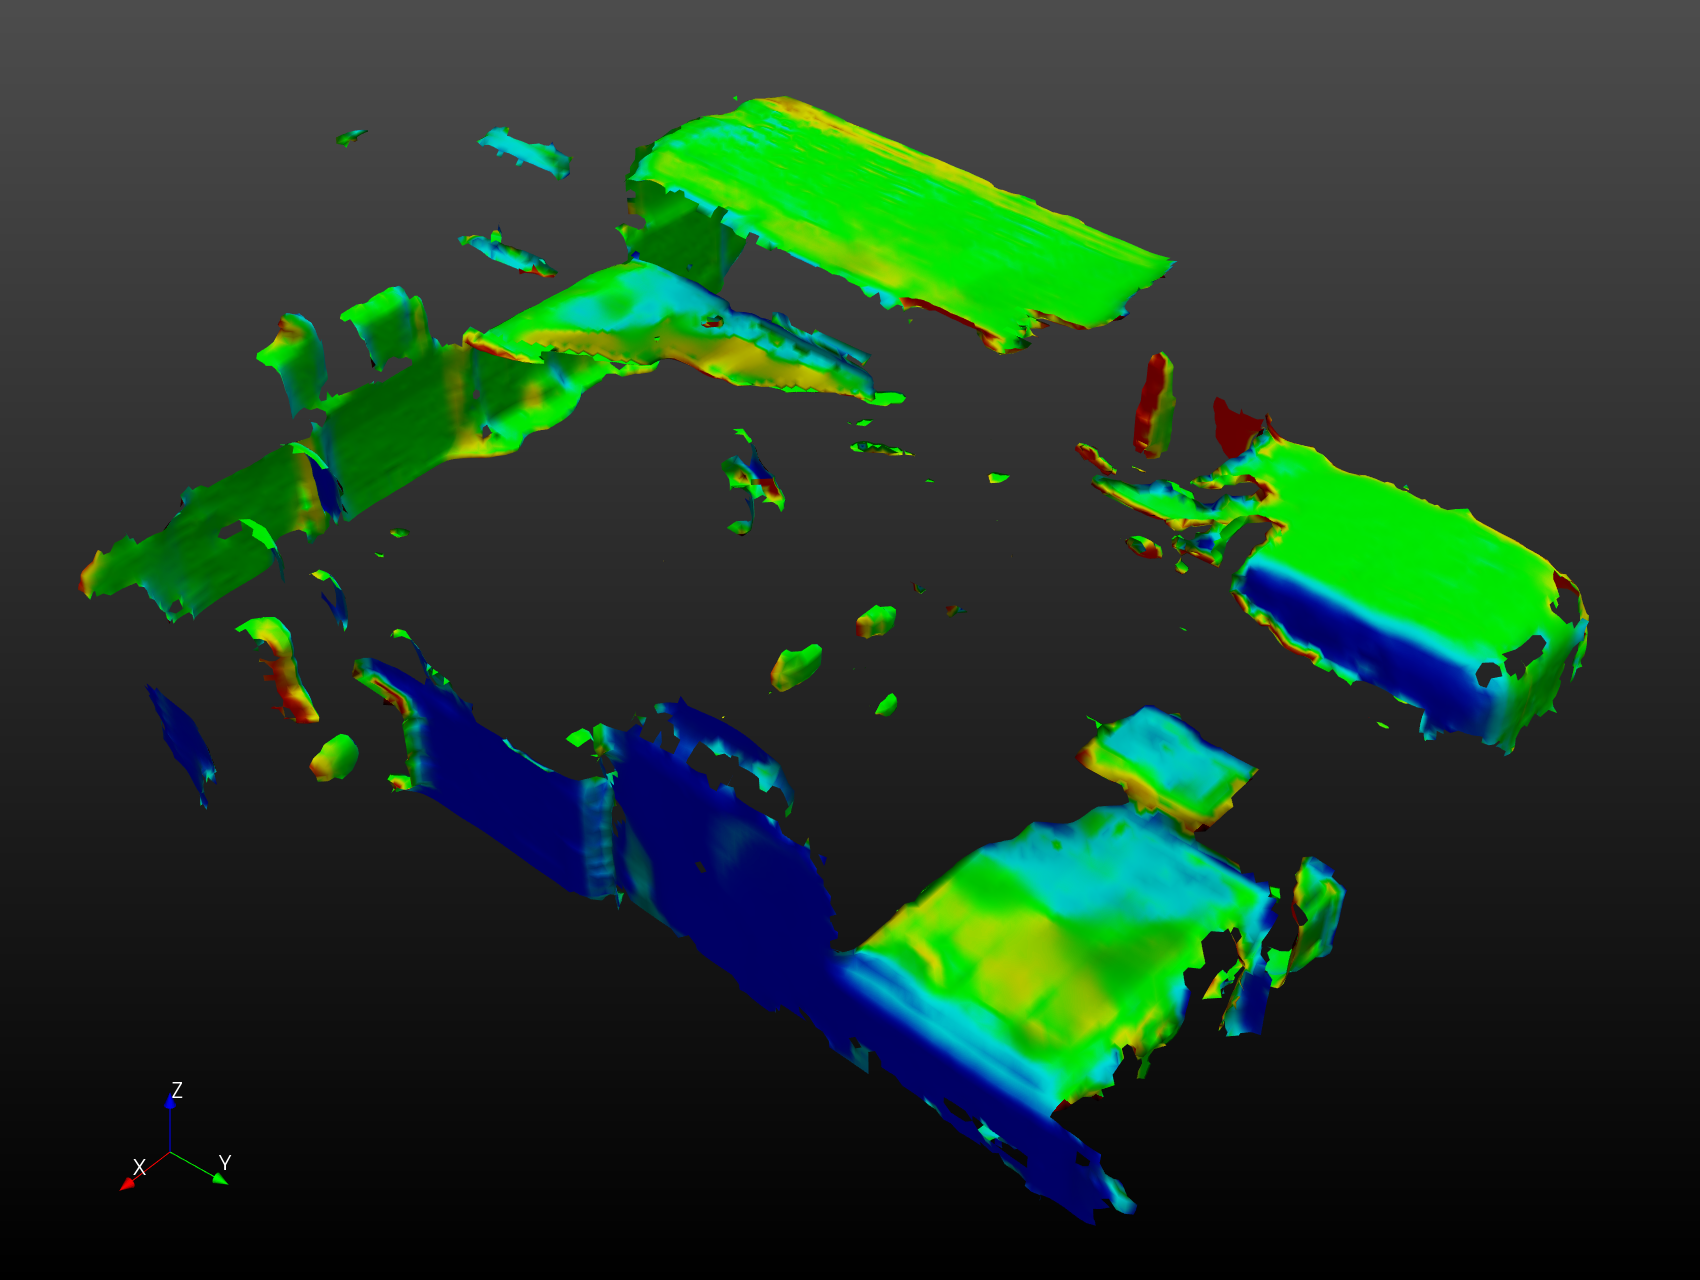
\includegraphics[width = 0.3\linewidth]{RegRec2N}} &
		\subfloat{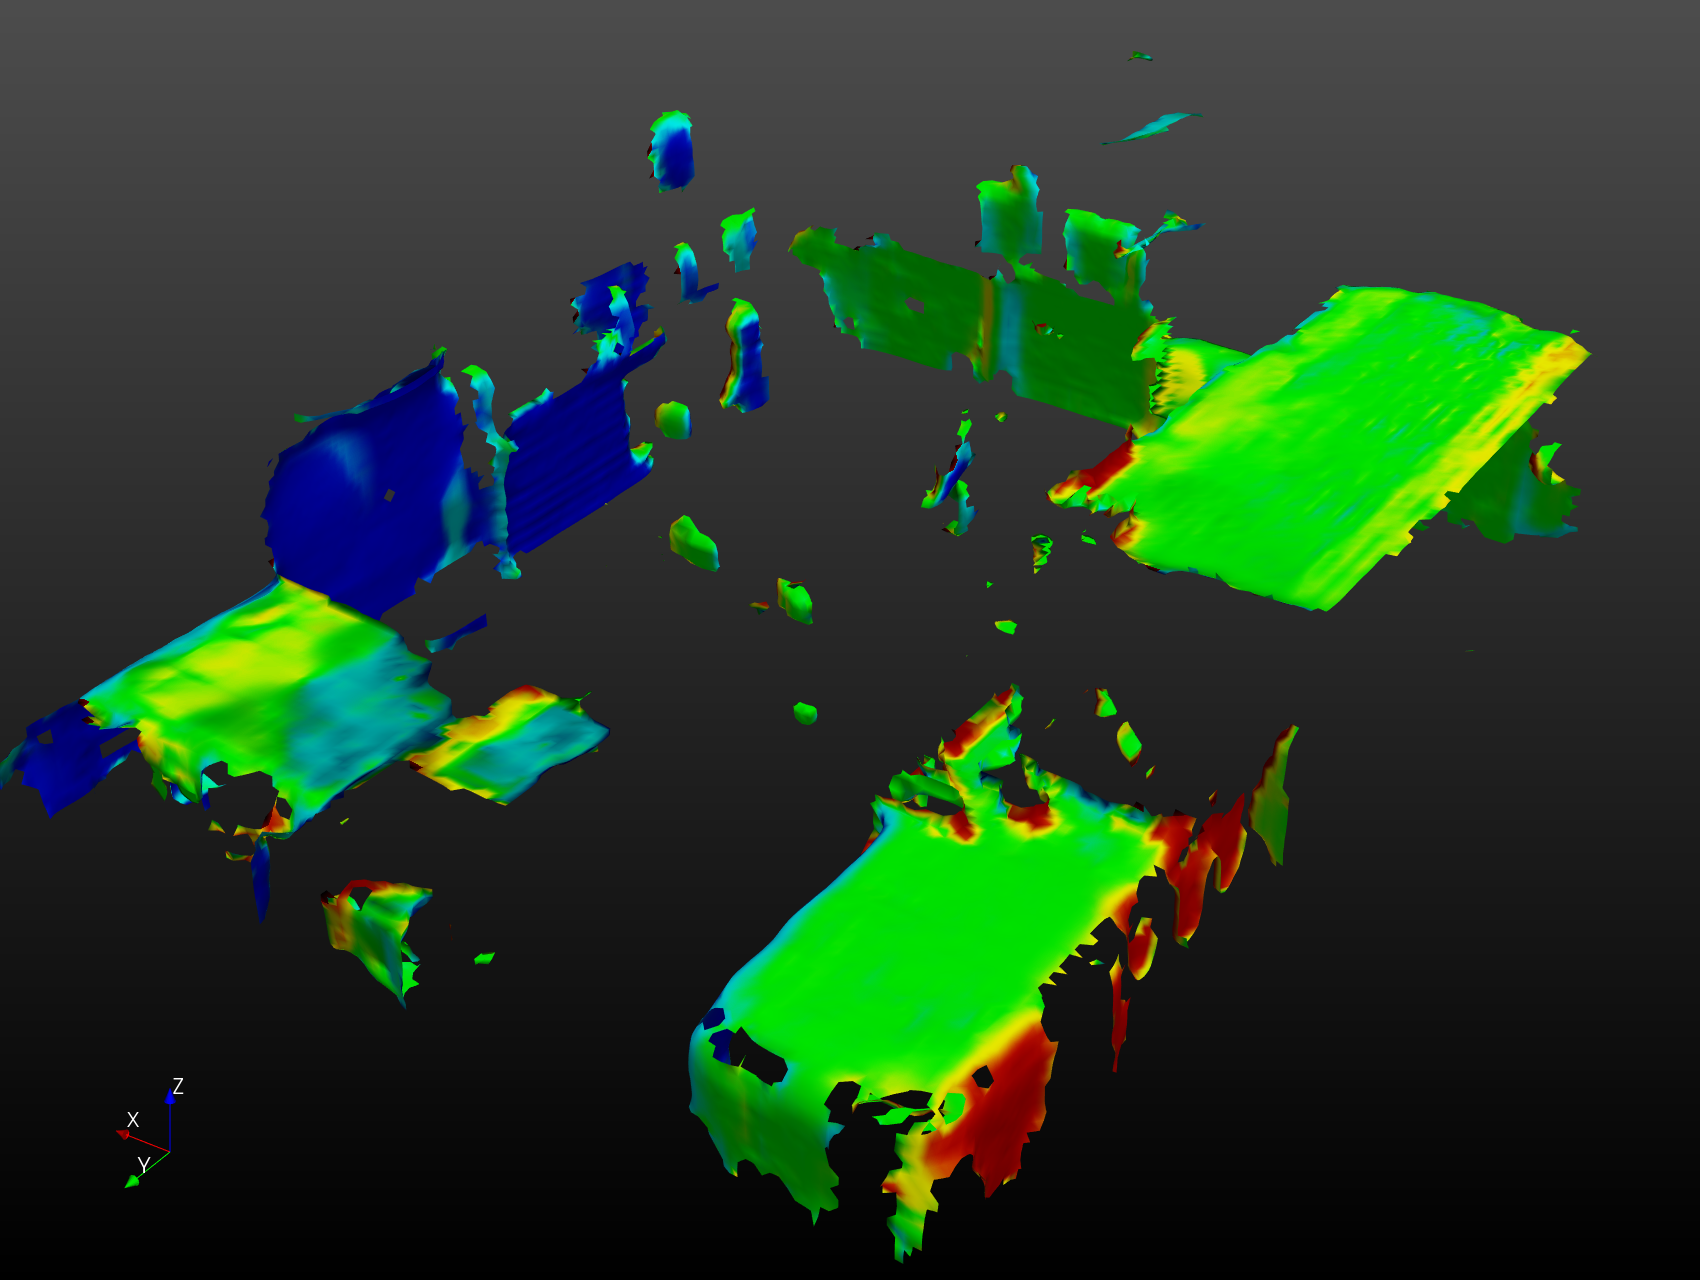
\includegraphics[width = 0.3\linewidth]{RegRec3N}}
		\end{tabular}
	\caption{Results of applying BORG CUBES to Point Clouds from first row. Second and Third Rows shows unregularized reconstruction (solid and normals coloured). Fourth and Fifth Rows show regularized reconstructions (solid and normals coloured)}
	\end{figure}	
	
	\newpage
	\section{Conclusion}

	\newpage
	\bibliography{4YPReportBibl}
	\bibliographystyle{ieeetr}

\end{document}
